\chapter{The Compact Muon Solenoid}
\label{chap:cms}
Centered at collision point 5 of the LHC, and located 100 meters below the town of Cessy, France, is an underground cavern that houses a particle detector called the Compact Muon Solenoid (CMS)~\cite{Breskin:1244506}~\cite{Chatrchyan:2008aa}. Weighing 12,500 tonnes and occupying a volume of 3600 cubic meters, CMS (shown in Fig. \ref{fig:CmsPulledApart}) is the most massive particle detector to be constructed at a collider experiment. The experimental collaboration that built, operates and uses the data collected by the detector is called the CMS collaboration, and comprises over 3000 participants from 199 institutions in 43 countries. 

The CMS detector was designed to study, among other things, particles produced through rare electroweak processes. At the LHC, such processes occur amid an overwhelming number of QCD dijet events (events with two  hadronic showers that recoil back-to-back) in an environment of high instantaneous luminosity. To reconstruct and identify particles amid the large background, the various sub-detectors of CMS measure various properties of the particles emerging from the collisions, and this information is used to form particle candidates. The properties that can be measured include the electric charge, energy, momentum, direction of motion, particle identity (ID), and the decay lifetime of particles. The ability to use information from the various sub-detectors to identify and characterize individual particles is made possible by CMS's fine granularity, meaning the sub-detectors are composed of small, closely-spaced units, or cells. The fine granularity is key to accurately measuring the position of particles passing through the detector, and minimizing the chances that the same cell will be activated by two particles simultaneously, which can complicate the reconstruction. This complication is enhanced by the fact that the high instantaneous luminosity of the LHC leads to, in most cases, the occurrence of multiple simultaneous collisions per bunch crossing rather than just a single collision, an effect called pile-up. A precise determination of the momentum of particles is made possible by a high magnetic field that fills the space of the inner sub-detectors, the tracker and electromagnetic calorimeter, described below. The global analysis of each event and its constituent particles is performed by an algorithm called particle flow \cite{Beaudette:2014cea}, some details of which are provided in the sections below.

\begin{figure}[h]
\centering
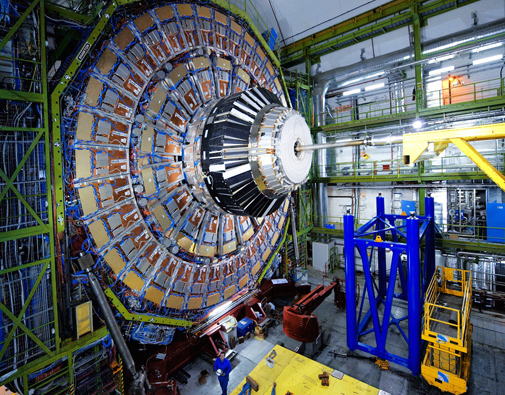
\includegraphics[width=0.6\linewidth]{figures/CMS/CMSBetter.jpg}
%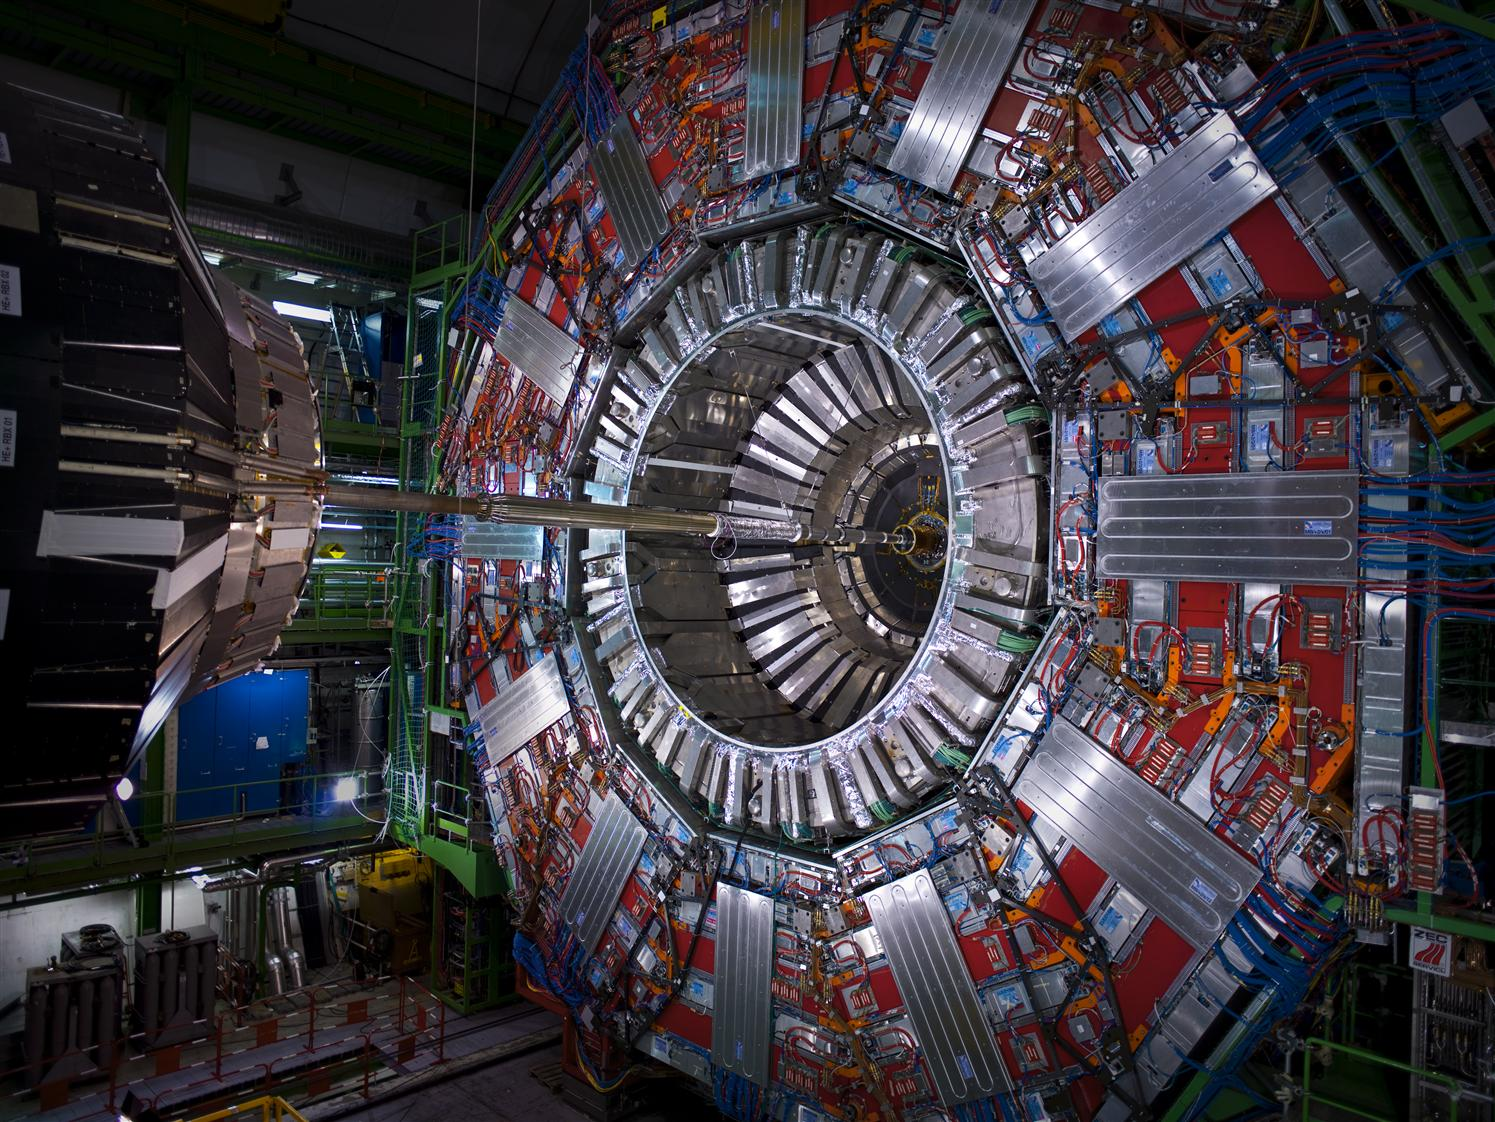
\includegraphics[width=1.0\linewidth]{figures/CMS/CMS1.jpg}
\caption{The CMS detector, pulled apart during the long shutdown of 2014. } 
\label{fig:CmsPulledApart}
\end{figure}
A photograph of the CMS detector is given in Fig. \ref{fig:CmsPulledApart}. The sub-detectors are nested cylindrically around the LHC beams, centered on the interaction point. A description of the coordinate system used by CMS, as well as a set of key observables that CMS is capable of reconstructing, is given in the following section. Then, the main systems are described, starting from the inside (closest to the beam lines) and moving outward.

\section{Coordinates and observables}
The CMS detector makes use of both a right-handed cartesian coordinate system as well as an approximately Lorentz invariant spherical coordinate system (HEP coordinate system). In the cartesian system, $\hat{x}$ points toward the center of the LHC, $\hat{y}$ points up, and $\hat{z}$ points in the direction of the counterclockwise rotation of the LHC beam pipe as viewed from above. The HEP coordinate system is spanned by the basis vectors $\pt$ (transverse momentum), $\eta$ (pseudorapidity), and $\phi$ (azimuthal angle), which translate to the right-handed cartesian coordinate system through the relations:
\begin{align}
\pt &= \sqrt{(p_{x})^2+(p_{y})^2}\\
\eta &= -\text{ln}[\text{tan}(\theta/2)]\\
\phi &= \hphantom{-}\text{tan}^{-1}(p_{\text{y}}/p_{\text{x}}),
\end{align}
where $\theta$ is the polar angle from the positive $\hat{z}$ axis.

The missing transverse momentum $\METvec$ is defined as the negative of the vector sum of the momenta of all visible particles in an event, projected on the plane transverse to the beam:
\begin{equation}
\METvec\!\equiv\!-\sum\limits_{i}^n(\vec{p}_T)_i.
\end{equation}
The $\METvec$ has magnitude $|\METvec|$, or just $\met$, and direction $\phimiss$, and is an estimate of the transverse momentum of the invisible particles. Since the true mass of an invisible particle is not observable, such masses are conventionally assumed to be zero, and the magnitude of the $\METvec$ vector is thus equated with the missing transverse energy \MET. The $\METvec$ can be used to construct the four-vector
\begin{equation}
(p_{\text{T}}^{\text{miss}})^\mu\equiv\!(E_T^{\text{miss}},\METvec)^\mu.
\end{equation}

Another key observable, $\Ht$, is a measure of the total hadronic energy in an event, and is defined as the scalar sum of the transverse momenta of jets in an event, or 
\begin{equation}
\Ht\!\equiv\!-\sum\limits_{i}^n(p_T)_i.
\end{equation}



\section{Silicon tracker}
The innermost system of CMS, immediately encountered by particles emerging from collisions, is the tracker \cite{Veszpremi:2014hpa}. Shown in Fig. \ref{fig:CmsTracker}, the tracker consists of two subsystems: a 600 cm-long inner pixel detector extending out to a radius of 11 cm, and a 5.8 m-long outer strips tracker extending out to a radius of 1.2 m.  The pixel detector is made of 66 million silicon pixels, and the strips detector contains 10 million silicon strips. The density of readout channels is highest within the innermost detector elements because the intensity of particle flux is highest in this region. Tracks left by muons (hadrons) are reconstructed with a very high efficiency of greater than 99\% (90\%) with a fake rate as low as 1\%, for transverse momenta as low as 150 MeV.
\begin{figure}[h]
\centering
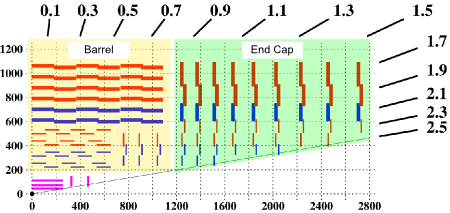
\includegraphics[width=0.75\linewidth]{figures/CMS/TrackerLayout.png}
\caption{A schematic view of the CMS tracker. The direction of view is toward the center of the LHC.} 
\label{fig:CmsTracker}
\end{figure}
At the design luminosity of the LHC of $10^{34}$ cm$^{-2}$s$^{-1}$, approximately 1,000 particles are created each 25 ns bunch crossing. This means that during the reconstruction, the innermost pixel layer is responsible for disentangling the tracks of about one million particles per mm$^2$ each second. The pixel detector is also responsible for resolving each particle's impact parameter, which is the distance of closest approach of the particle's trajectory to the point of the proton-proton collision, which is called the primary vertex. This task will be particularly challenging when the LHC enters its high luminosity phase, since the occurrence of multiple collisions within the same bunch crossing, will become much more prevalent. 

\section{Electromagnetic calorimeter}
Upon reaching the outer edge of the CMS tracker, particles enter the electromagnetic calorimeter (ECAL). The ECAL is made of 72,000 lead tungstate (PbWO$_4$) crystals, like the one shown in Fig. \ref{fig:CmsTracker}. 
\begin{figure}[h]
\centering
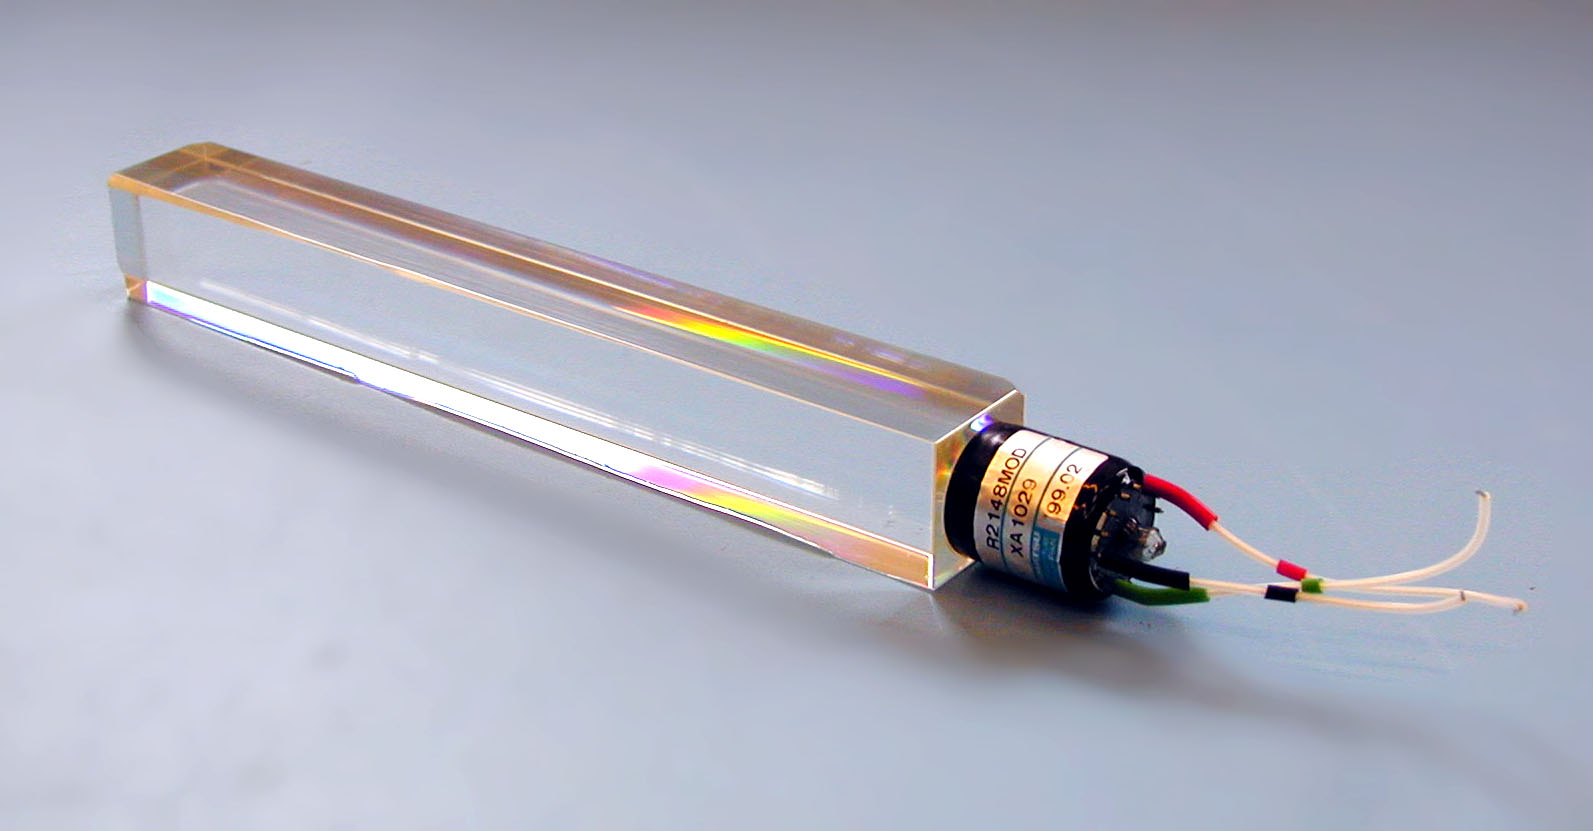
\includegraphics[width=0.75\linewidth]{figures/CMS/PbWO4.jpg}
\caption{An ECAL endcap PbWO$_4$ crystal, length 220 mm (24.7 X$_0$).} 
\label{fig:CmsTracker}
\end{figure}
The material was chosen for its high density and high optical transparency, which, respectively, guarantee a short radiation length (X$_0$ = 0.89 cm) and efficient transmission of light. Highly-relativistic charged  particles emit bremsstrahlung radiation as they traverse the crystals, resulting in electromagnetic showers, and the light is collected by photodetectors mounted on the backs of the ECAL crystals. The amount of radiation produced is proportional to the energy of traversing particles, which key to determining the energy of particles during the event reconstruction. PbWO$_4$ is also chosen for its small Moli\`{e}re radius of 2.2 cm, which results in an improved spatial resolution of particles over that possible with other materials.
\begin{figure}[tb!]
\makebox[\textwidth][c]{
\centering
\subfloat[]{
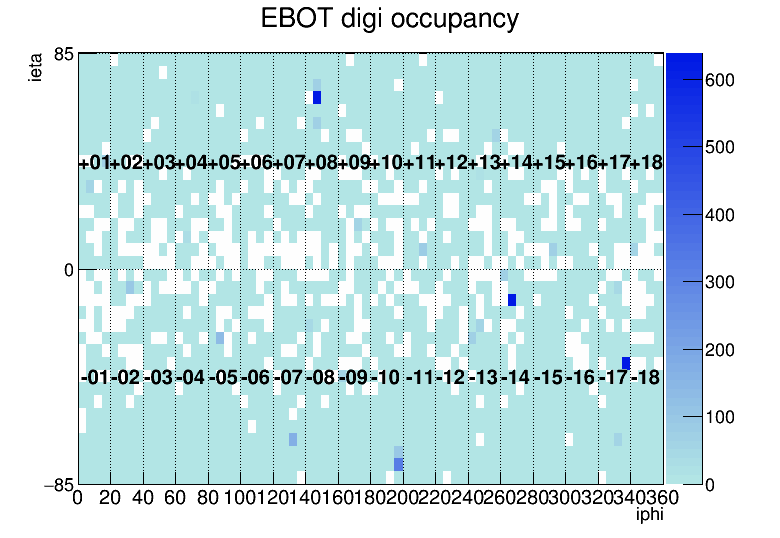
\includegraphics[width=0.7\linewidth]{figures/CMS/EBOccupancy.png}
}
}
\makebox[\textwidth][c]{
\centering
\subfloat[]{
  \vspace{2cm}
  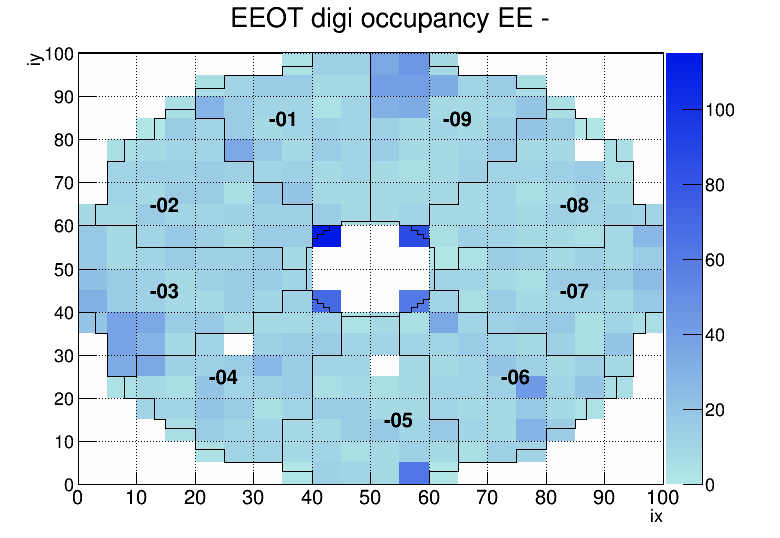
\includegraphics[width=0.5\linewidth]{figures/CMS/EB-Occupancy.png}
  }
  \subfloat[]{
  \vspace{2cm}
  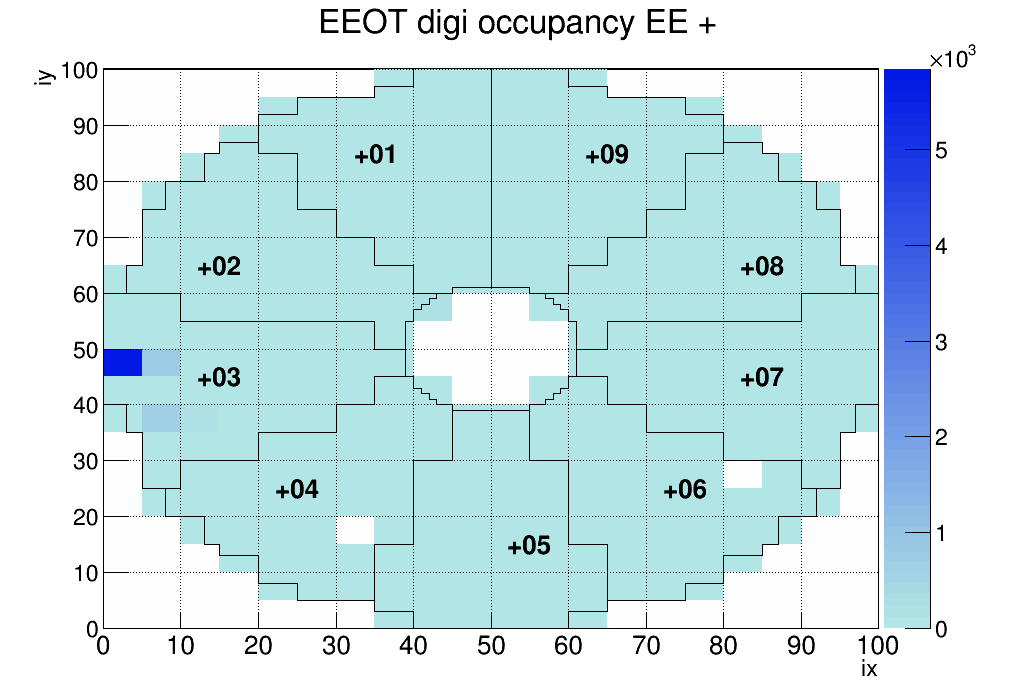
\includegraphics[width=0.5\linewidth]{figures/CMS/EB+Occupancy.png}
}
}
\caption{The layout of the ECAL barrel (a) in $\eta$-$\phi$ coordinates, and the forward (c) and rear (b) ECAL endcaps in cartesian coordinates. The shading shows the occupancy of a given run. OT stands for out-of-time, indicating that the occupancy shown in the color plot is of energy deposits that were detected out of time with the LHC bunch crossings.} 
\label{fig:EcalLayout}
\end{figure}

In the barrel, crystals are organized into rectangular modules composed of 400 or 500 crystals each, and modules are arranged in groups of four to form supermodules. There are 36 supermodules in total, which combine to cover a large rectangular area in the space of $\eta$ and $\phi$, as shown in Fig. \ref{fig:EcalLayout} (a). This large rectangle covers all values of $\phi$ and reaches an $\eta$ of $\pm$ 1.48. In the endcaps, crystals are arranged in groups whose number varies depending on the location. The modules combine to form sectors, of which there are a total of 18, shown in Fig. \ref{fig:EcalLayout} (b) and (c). Sectors, as well as supermodules, are each read out by a front end digitizer (FED).

Deposits in the calorimeters are analyzed in the reconstruction to yield calorimeter clusters. A calorimeter cluster is composed of cells corresponding to a relative maximum in the amount of energy deposited, and the cluster energy is equal to the energy deposited in the central cell summed with the energy deposited in neighboring cells, provided that a neighboring cell has an energy deposit exceeding 1 GeV. The ECAL is capable of determining the energy of photons and electrons with a resolution of 1$-$5\%, depending on the pseudorapidity, and charged hadrons with a resolution of about 10\%. 



\subsection{ECAL calibration}
Ensuring an equivalent and accurate response among the various crystals (channels) requires a detailed calibration procedure. The ECAL is calibrated {\it in situ}, or while the detector is operating, and a number of methods are employed. The first method exploits the the principle of the $\phi$-invariance of collisions. Since the primary proton beams are unpolarized, outgoing particles are distributed isotropically in the azimuthal angle $\phi$, and this allows channels with different $\phi$ locations but within a small $\eta$ region to be checked against one another. The second method, which is the most important, relies on the tracker to give an accurate estimate of the momentum of isolated electrons. The momentum of the tracks can be used to scale the response of the ECAL signal to the appropriate value. This method makes use of electrons from events in which a W boson is produced and decays to e + $\nu_{\text{e}}$, in which the outgoing electrons exhibit a broad $p_T$ spectrum that peaks around 40 GeV. The third method employs tag and probe methods~\cite{Beaudette:2014cea} in which neutral mesons decay to two $\gamma$ particles. 

The second method relies on the clean measurement of the momenta of electrons from the tracker, but as will be explained in Section \ref{sec:Trigger}, information from the tracker is not available to the CMS level 1 (L1) trigger (Section \ref{sec:Trigger} gives a description of the L1 trigger). Therefore, the collection (triggering) of events to be used for calibration must rely on information from the ECAL itself, as well as the hadronic calorimeter (HCAL), the system described in the next section. It is crucial to ensure that enough events with low-energy electrons are triggered in order to calibrate the ECAL, while preventing the large background of charged pions from overwhelming the calibration sample. For this, a selection is applied to events containing e/$\gamma$ candidates, which is a collection of four-vectors that contain nearly all electrons and charged pions. The goal is to discriminate between the pion background and the electrons to be used for calibration, and ultimately reject as many candidates believed to be pions as possible, while reconstructing enough electrons to calibrate the ECAL. The fundamental triggering information used in the selection are the called trigger primitives, and are:
\begin{itemize}
\item et2x1: the energy of the e/$\gamma$ candidate, equal to the summed energy deposited in the two adjacent ECAL trigger towers, which are $5\times5$ arrays of crystals, closest to the crystal with maximum energy deposit.
\item et12x12: the energy of a jet candidate, equal to the sum of all ECAL and HCAL energy in the 12$\times12$ array of trigger towers surrounding the e/$\gamma$ candidate, multiplied by 4.
\end{itemize}
The simulated distributions of these primitives for signal and background e/$\gamma$ candidates is shown in Fig. \ref{fig:TriggerObservables} (a), where a proximity matching has been applied between the e/$\gamma$ candidates and the parton-level, often referred to as ``truth"-level, particles.  These primitives are the building blocks of observables designed to give good signal/background discrimination when used in a cut-based, that is, threshold-based, selection, which are:
\begin{itemize}
\item hadronic energy fraction (H/E): The ratio of the energy deposited in the of the 3x3 array of HCAL towers centered on the e/$\gamma$ seed to that deposited in the corresponding 3x3 array of ECAL towers:
\begin{equation}
\text{H/E} = \sum_{3\times3}{\text{HCAL}}/\sum_{3\times3}\text{ECAL};
\end{equation}
\item isolation: The sum of the energy deposits surrounding the ECAL seed divided by the energy of the seed:
\begin{equation}
\text{isolation} = (0.25\times\text{et12x12} - \text{et2x1})/\text{et2x1}.
\end{equation}
\end{itemize}
Simulated distributions of these observables are shown for signal and background e/$\gamma$ candidates in Fig. \ref{fig:TriggerObservables} (b). 
\begin{figure}[tb!]
\makebox[\textwidth][c]{
\centering
\subfloat[]{
  \vspace{2cm}
  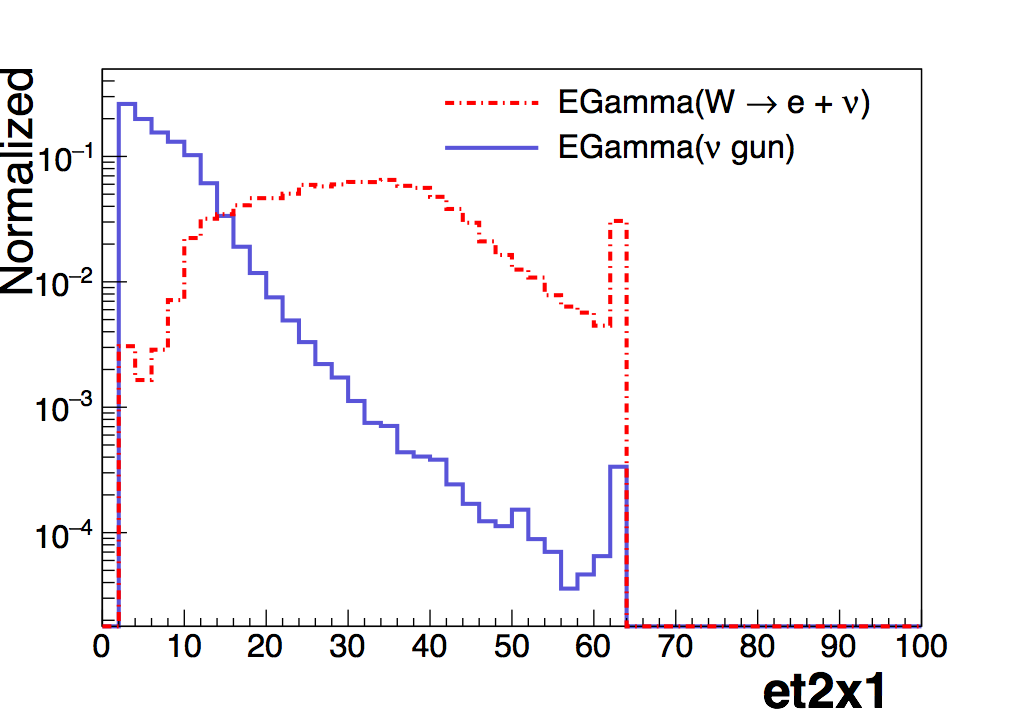
\includegraphics[width=0.5\linewidth]{figures/CMS/ECALPrimitives1.png}
    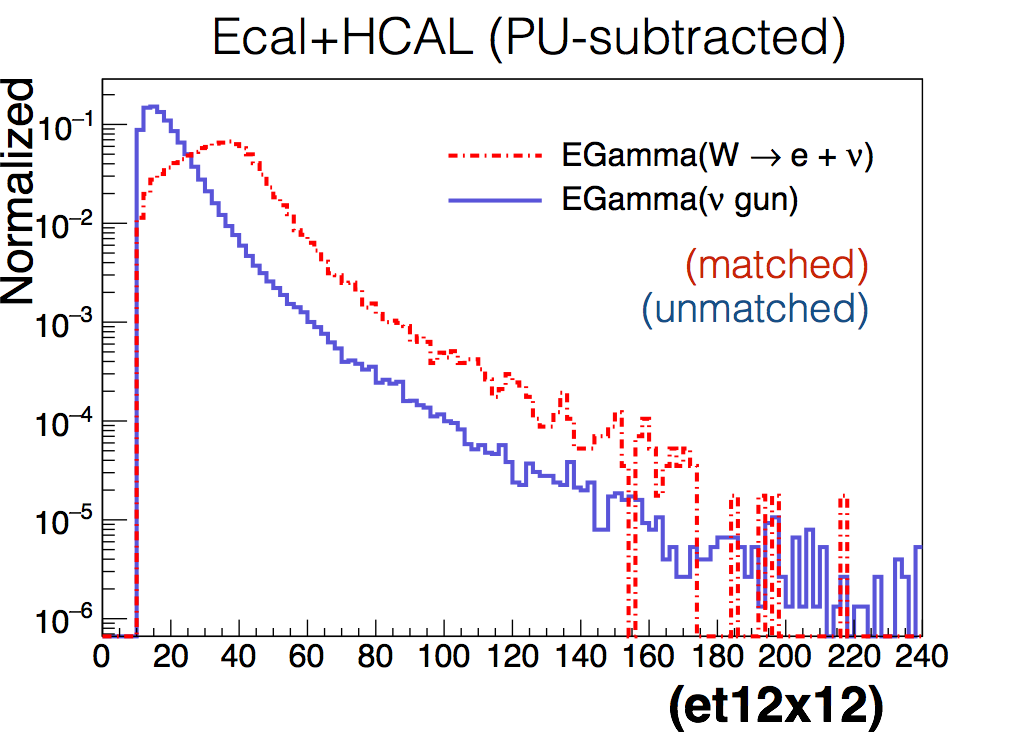
\includegraphics[width=0.5\linewidth]{figures/CMS/ECALPrimitives2.png}
  }
  }
  \makebox[\textwidth][c]{
  \subfloat[]{
  \vspace{2cm}
  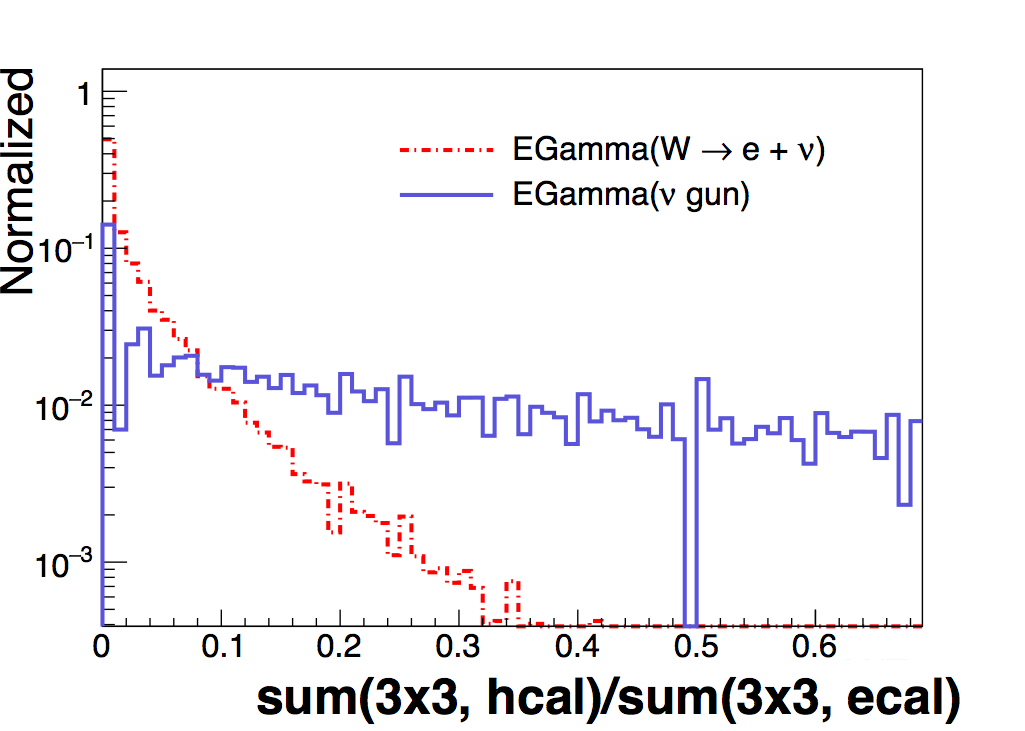
\includegraphics[width=0.5\linewidth]{figures/CMS/ECALHoE.png}
    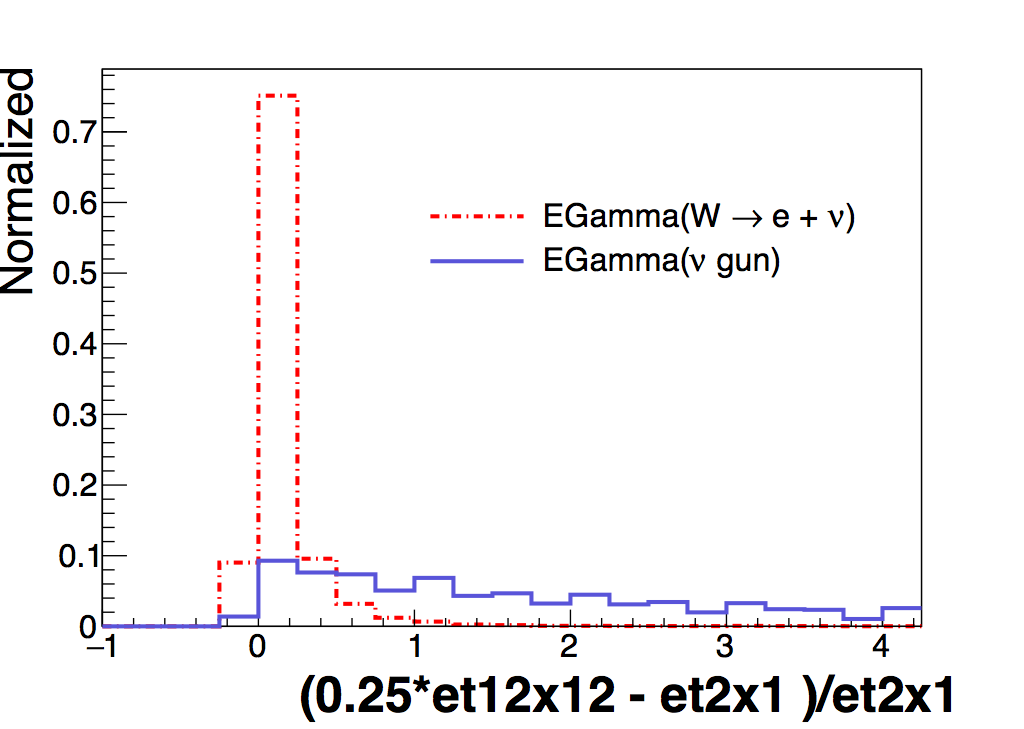
\includegraphics[width=0.5\linewidth]{figures/CMS/ECALIso.png}
}
}
\caption{The trigger primitives available from the calorimeters available to the CMS L1 trigger (a), and the observables derived from the primitives designed to discriminate between signal and background e/$\gamma$ candidates.} 
\label{fig:TriggerObservables}
\end{figure}

The efficiency, or fraction of e/$\gamma$ candidates matched to true electrons that are selected by the baseline selection of 
\begin{itemize}
\item isolation < 2.0
\item H/E < 0.5,
\end{itemize}
is shown in Fig. \ref{fig:EGammaEfficiencies} for various thresholds, shown in the figure.
\begin{figure}[h]
\makebox[\textwidth][c]{
\centering
  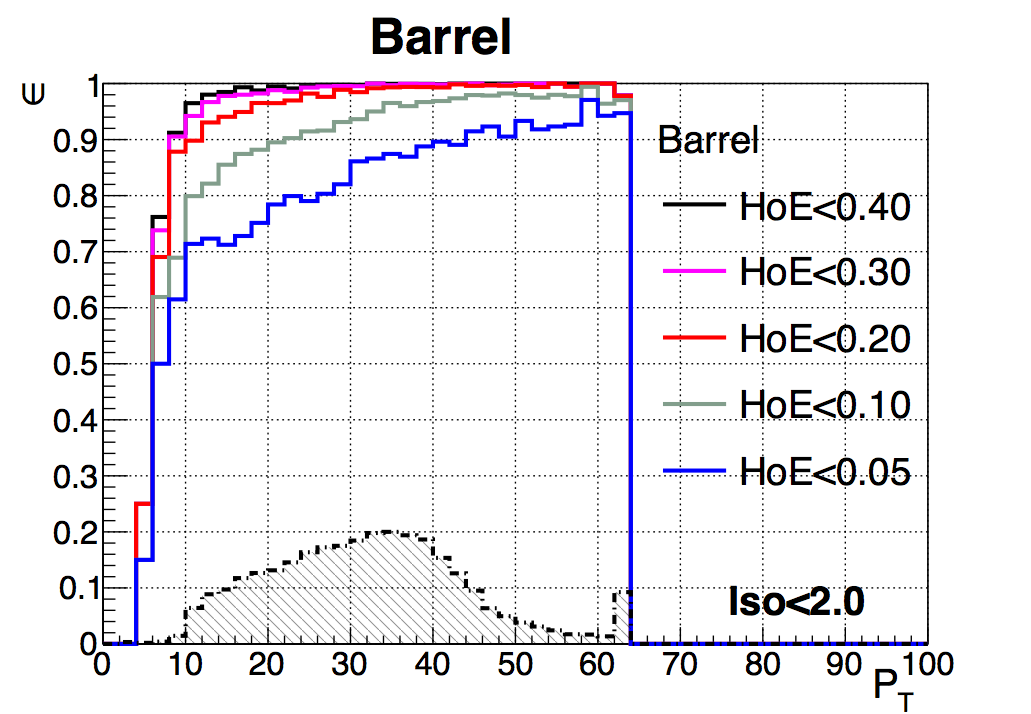
\includegraphics[width=0.49\linewidth]{figures/CMS/EcalEffIsoBarrel.png}
  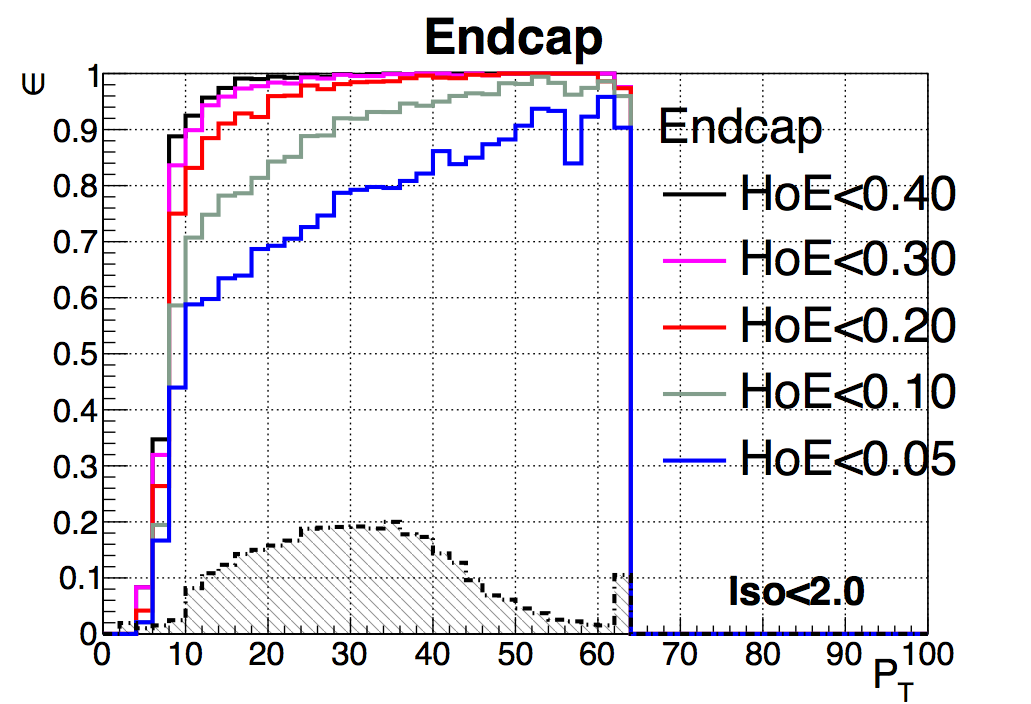
\includegraphics[width=0.49\linewidth]{figures/CMS/EcalEffIsoEndcap.png}
  }
  \makebox[\textwidth][c]{
\centering
  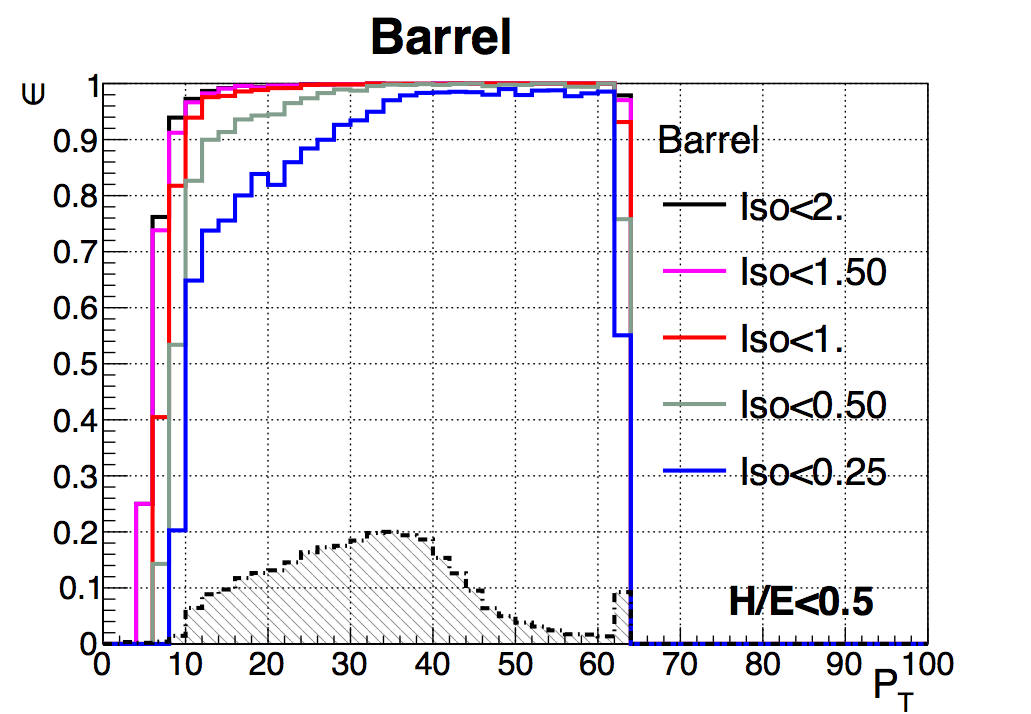
\includegraphics[width=0.49\linewidth]{figures/CMS/EcalEffHoEBarrel.png}
  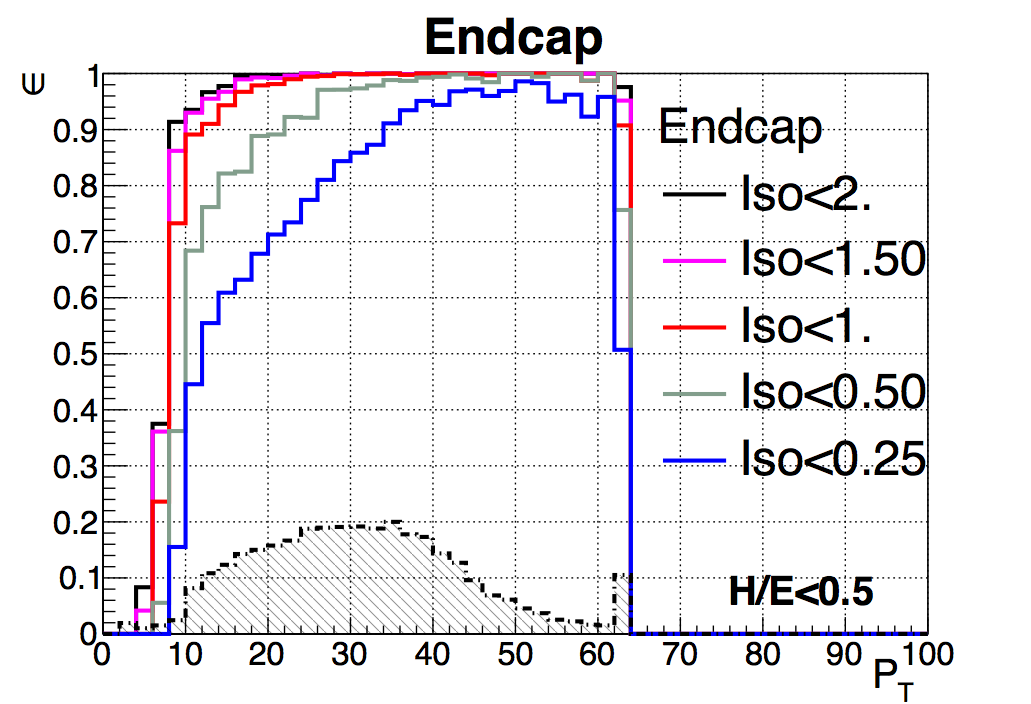
\includegraphics[width=0.49\linewidth]{figures/CMS/EcalEffHoEEndcap.png}
}
\caption{The signal efficiency in the barrel and endcap as a function of the $p_T$ of the e/$\gamma$ candidates for various thresholds on the H/E and isolation.} 
\label{fig:EGammaEfficiencies}
\end{figure}

The performance of the currently applied cut-based selection was investigated by comparing the existing performance with that obtained through the use of an idealized discriminator. The idealized discriminator chosen was a boosted decision tree (BDT)~\cite{Hocker:2007ht} whose input variables are the observables H/E and isolation. The BDT was trained using half of the available simulated signal candidates and half of the background candidates, while half of both collections was set aside as an independent test sample. Figure \ref{fig:ECALMva1} characterizes the performance of the cut-based and BDT selection, showing the trade-off between the signal efficiency and background contamination in the test sample. The performance of the idealized discriminant is comparable to the performance of the selected working points of the cut-based approach, indicating that the values of the currently-employed selection is well-optimized. 
\begin{figure}[h]
\centering
  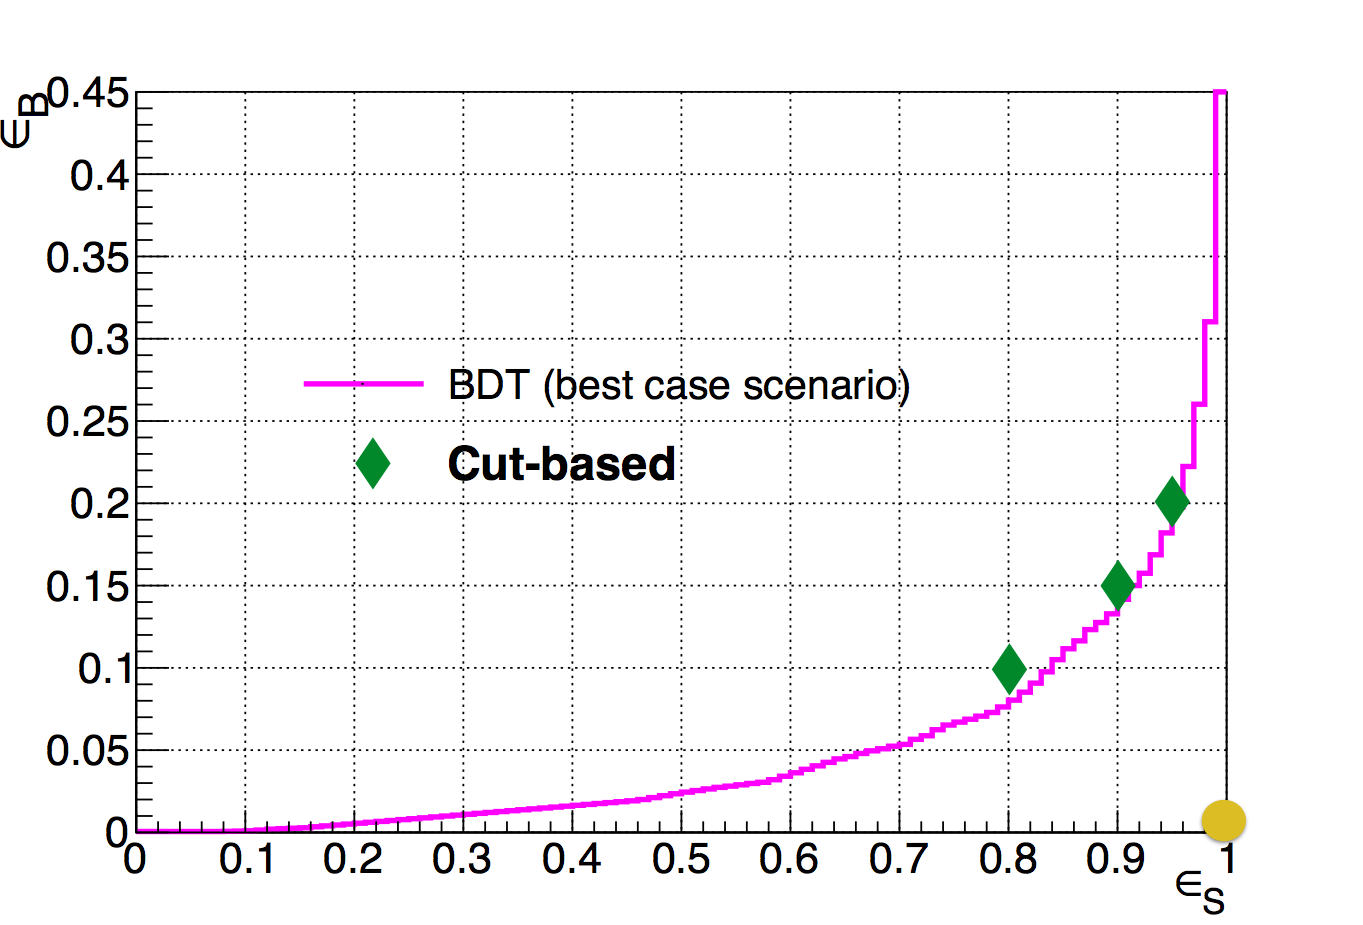
\includegraphics[width=0.79\linewidth]{figures/CMS/ECALMva1.png}
\caption{The background efficiency vs the signal efficiency for cut-based selection and the selection of the BDT based whose inputs are the cut-based observables. The ideal point is indicated by the gold circle located at full signal efficiency and zero background efficiency. For a given background efficiency, the cut-based signal efficiency is within a few percent of the BDT efficiency.}
\label{fig:ECALMva1}
\end{figure}

The addition of new observables in the selection was also investigated. For example, the centrality, explained in  called the centrality, explained in Fig. \ref{fig:centrality}
\begin{figure}[h]
\centering
  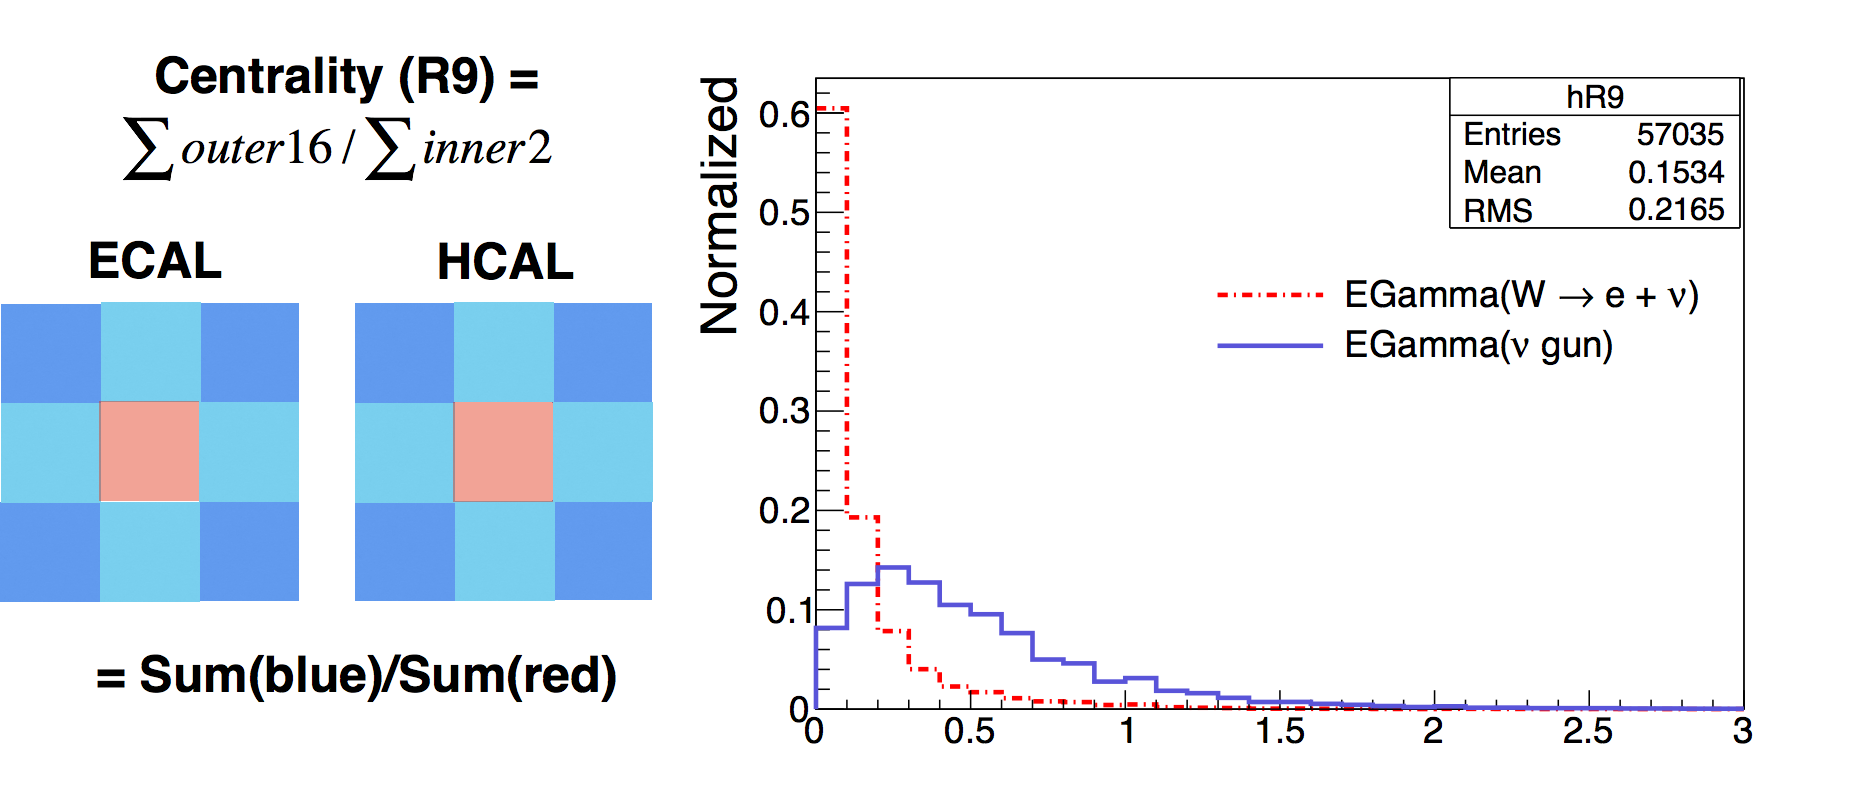
\includegraphics[width=0.95\linewidth]{figures/CMS/EcalCentrality.png}
\caption{The definition of the centrality (left), along with the distributions of the centrality for signal and background e/$\gamma$ candidates in simulation (right). }
\label{fig:centrality}
\end{figure}
The change in performance of the BDT with the centrality is shown in Fig. \ref{fig:ECALMva3}. Including the centrality improves the performance by about 10-15\%, which implies a 10-15\% reduction in the background rate  for a given signal efficiency. This result has been presented to the ECAL DPG working group and is available if a 10-15\% reduction in the trigger rate is required for calibrating in subsequent runs. A cut-based selection on this observable would need to be applied, since the use of multivariate discriminants is not possible, at present, in the L1 trigger.
\begin{figure}[h]
\centering
  \includegraphics[width=0.79\linewidth]{figures/CMS/ECALMva3.png}
\caption{The background efficiency vs the signal efficiency for cut-based selection, the plane BDT selection, and the selection of the BDT trained with the addition of the centrality variable. The ideal point is indicated by the gold circle located at full signal efficiency and zero background efficiency. For a given signal efficiency, a suppression of the background on the order of 10-15\% is possible. }
\label{fig:ECALMva3}
\end{figure}


\section{Hadronic calorimeter}
Immediately surrounding the CMS ECAL and inside the CMS solenoid magnet is a sampling hadronic calorimeter (HCAL), shown in Fig. \ref{fig:HCalLayout}. Constructed from plates that alternate between steel, brass, and plastic scintillating material, the HCAL comprises a barrel with 36 azimuthal wedges covering the range $|\eta|<1.3$, and two endcaps covering the range $1.3<|\eta|<3$. The number of interaction lengths ($\lambda_{0}$) in the barrel ranges between 5 to 10 $\lambda_{0}$, and about 10 $\lambda_{0}$ in the endcaps. The geometry of the 36 barrel wedges closely matches the geometry of the 36 ECAL supermodules. An individual HCAL cell subtends the solid angle of a $5\times5$ array of ECAL crystals. The geometry of the endcaps differs from that of the ECAL.
\begin{figure}[h]
\centering
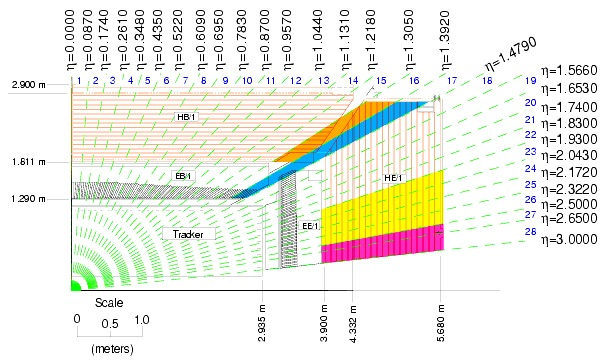
\includegraphics[width=0.95\linewidth]{figures/CMS/HCalLayout.jpg}
\caption{A schematic view of the CMS HCAL. The direction of view is toward the center of the LHC.} 
\label{fig:HCalLayout}
\end{figure}


\section{Superconducting solenoid}
Dividing the inner detector from the outer is a 12-m long, 6-m-diameter superconducting solenoid magnet, the system most critical for the functionality of the CMS detector. Niobium Titanium coils, kept at a temperature of 3.2 K and carrying a stored energy of 2.6GJ, are responsible for filling the inner detector with a uniform 3.8 T magnetic field. The superconducting coils are cooled by liquid helium that is supplied and cooled via a multistage cryogenic system that is managed by the External Cryogenics Group of the LHC. Oil contamination in this system resulted in sub-optimal performance of the CMS solenoid in 2015, and led to a 20\textemdash30\% loss in the data collected.

 
\section{Muon system}
The outermost subdetector of CMS is the muon system. The rest of the CMS detector, 
which is nested within the muon systems, amounts to 16 interaction lengths of material, 
and so the only particles that are able to interact with the muon system are muons. Like 
the other subdetectors, the muon system coheres to the azimuthal symmetry of the CMS 
solenoid. Composed of a barrel and two endcaps, the muon system provides complete 
pseudorapidity coverage in the range $|\eta|<2.4.$ The muon detector, shown in Fig. 
\ref{fig:MuonSystem}, is made of 4 concentric, cylindrical stations, and each station is 
composed of 12 ionizing drift chambers~\cite{Breskin:1244506}. On its own, the muon system 
is capable of determining the momentum of muons with a $p_{\text{T}}$ of up to 1 TeV with 
a resolution of 15\% in the barrel and 40\% in the endcaps. When utilizing information from 
both the muon system and the inner tracker, muon momentum can generally be determined 
to within 5\%.
\begin{figure}[h]
\centering
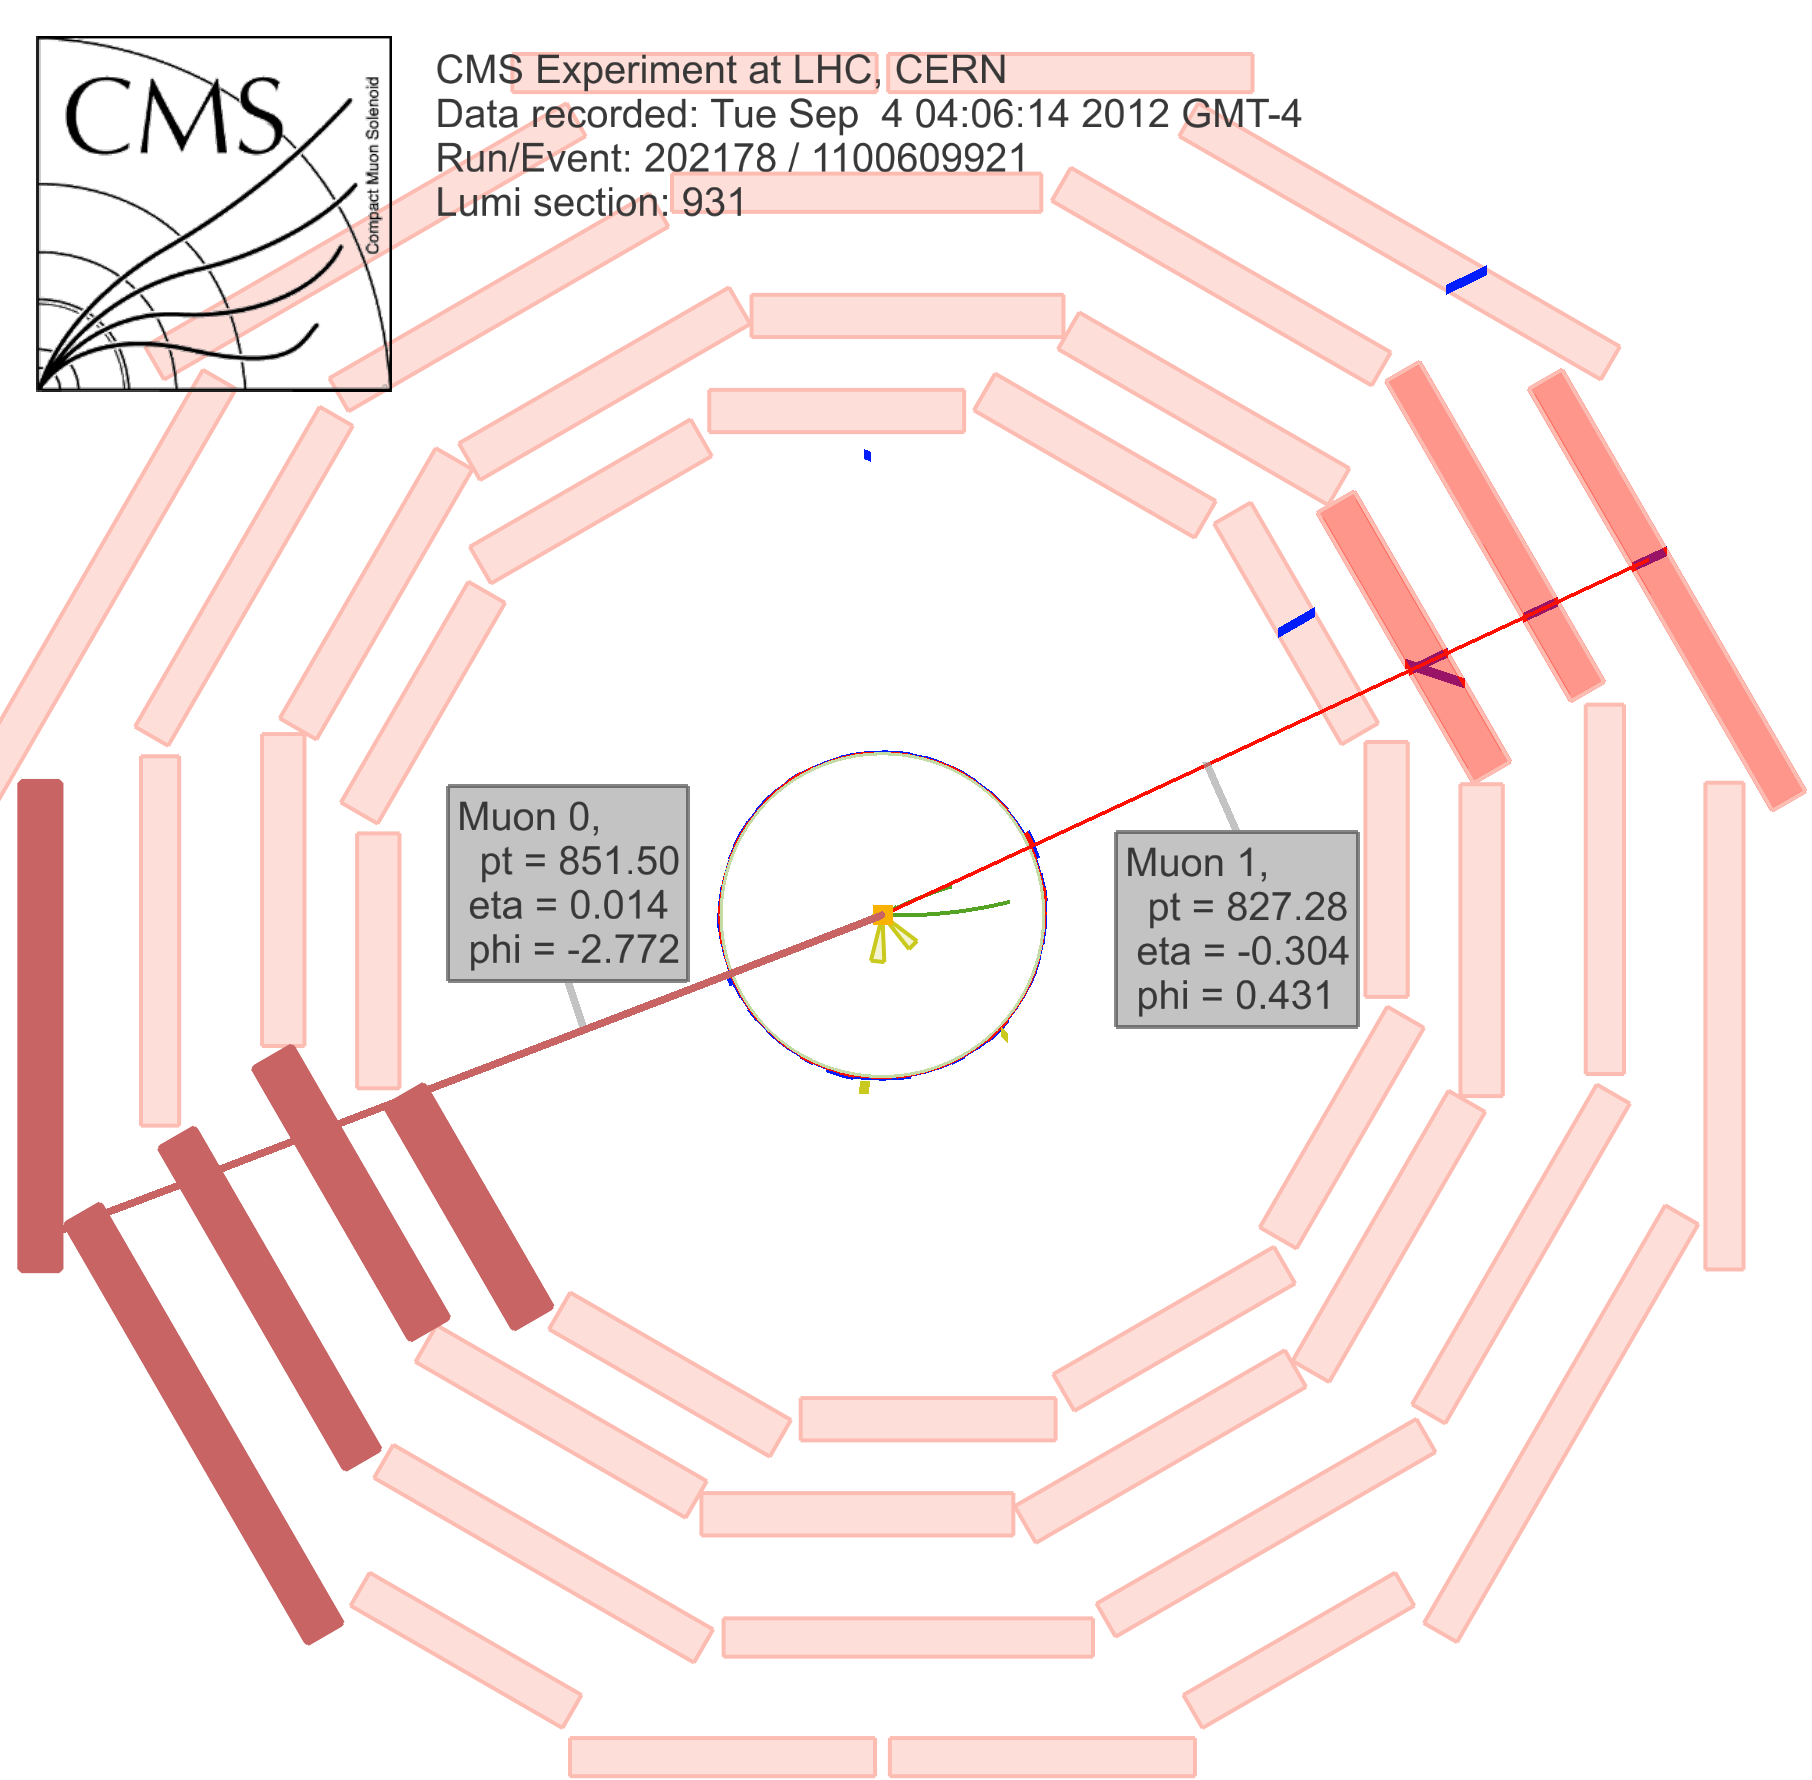
\includegraphics[width=0.5\linewidth]{figures/CMS/MuonSystem.png}
\caption{An event display of the CMS muon system. Two muons are reconstructed in the muon system.} 
\label{fig:MuonSystem}
\end{figure}

\section{Trigger and DAQ}
\label{sec:Trigger}

The two most critical components for the CMS detector to take data are the trigger and the data acquisition system (DAQ).  The trigger's purpose is to analyze one billion proton-proton collisions per second and quickly decide which events are to be written to disk, and which are discarded. Because of the finite computing speed and storage capacity, a maximum of about 1000 collision events per second can be recorded. Therefore, the vast majority of collisions are never reconstructed.

In order to reduce the number of events by 6 orders of magnitude, CMS employs a two-level trigger system. The two logically sequential trigger stages are: the level-1 (L1) trigger, and the high level trigger (HLT), each of which lowers the rate of events by a factor of a thousand. The L1 trigger is based on custom-manufactured programmable electronics and is responsible for analyzing each collision immediately after every bunch crossing, and discarding 99.9\% of the events. This trigger has access to coarse information from the calorimeters and muon system, namely, energy deposits in the calorimeters and hits in the muon chambers, collectively called trigger primitives. The L1 trigger uses these primitives to compute estimates of the four-vectors of $\mu$ candidates and e/$\gamma$ candidates, as well as estimates of the $\Ht$ and $\met$. The L1 trigger is allowed about 3 $\mu$s to analyze each event, and if it accepted, the event is passed to the HLT. 

The HLT, which is based in software, is capable of analyzing events with a much greater degree of sophistication than the L1. The information available to the high level trigger includes information from the CMS tracker, finely-granulated calorimetric depositions, and global objects that are constructed from the combination of all detectors.  The determination of the objects such as the $\Ht$ and $\met$ is much more precise in the HLT than in the L1, but less precise than the in the offline reconstruction.  Thus, at the analysis level, the trigger efficiency must be measured using the offline information.

The DAQ is the computer system responsible for storing information about events that have been accepted by the trigger. It is capable of processing 100 Gigabytes, or 100 events per second on average. The DAQ  integrates and analyzes the signals from about 55 million channels within the CMS detector, which are sent from about 600 independent front-end readout drivers. After processing, the DAQ sends the event information into mass storage on the CMS Tier-0 computing  enter, hosted by the CERN Data Centre.

\section{Particle and event reconstruction}
\label{sec:reconstruction}
The reconstruction of particles and event-level observables is performed by the particle flow algorithm~\cite{Beaudette:2014cea}. Particle flow analyzes the basic elements from each detector system (tracks in the tracker, calorimeter clusters, and muon tracks), and associates the elements to form single particle candidates. The final result is a global event description that attempts to characterize every particle in each event. Jets and event-level observables such as the missing transverse energy $\met$ are constructed from these particles. 

Muons are identified based on information from the muon system and the inner tracker.  Specifically, a muon is identified as a track in the muon system that is consistent in energy and direction with a track in the inner tracker. A selection is made on the $\chi^2$ of a fit of the muon track to the combined hits in the tracker and muon system, and the momentum estimated by the muon system is required to fall within three standard deviations of the estimate made by the tracker.  

Electrons are identified as tracks in the inner tracker that are spatially and energetically consistent with energy clusters in the ECAL. Because electrons can emit photons when traversing the tracker, their trajectories can exhibit abrupt changes. Therefore, a special tracking algorithm called a Gaussian Sum Filter~\cite{Beaudette:2014cea} is used to model the trajectories of electron tracks in a realistic way. The algorithm that reconstructs energy clusters in the ECAL accounts for photon emission by identifying energy deposits consistent with possible trajectories of emitted photons, and adding them to the total cluster energy.  After the track is associated with an ECAL cluster, information from the ECAL and tracker is used to identify electrons, including the quality of the fit associated with the reconstructed track,  properties related to the distribution of the energy deposited in the ECAL, the ratio of the energy deposited in the HCAL behind the relevant ECAL cluster to that deposited in the ECAL, and the individual momentum estimates from the tracker and ECAL. Charged hadrons are identified as the set of track candidates matched to ECAL clusters that did not pass the electron identification criteria. 

Photons are identified in a similar manner as electrons, but it is required that no track point in the direction of the electromagnetic energy cluster, and little or no energy deposited in the HCAL. Remaining energy deposits in the HCAL are identified as neutral hadrons. 

The result of the above algorithm is a set of particles, called particle flow candidates, representing all identified particles in the event. Jets are reconstructed by applying the anti-k$_{\text{T}}$ algorithm \cite{Cacciari:2008gp}, with a distance parameter of 0.4 or 0.5, to the particle flow candidates. Estimates of the jet energy are corrected for effects of pile-up and for non-uniformities in the detector. The jet energy resolution ranges from 5$-$20\%, depending on the jet momentum and direction. The $\met$ is computed as the magnitude of the vectorial sum of the four-momenta of all particle flow candidates and jets in the event, after the energy corrections have been applied to the jets.

\label{sec:Trigger}


\section{Phase II upgrade}
In the year 2023, the high luminosity LHC (HL-LHC) will begin operations of what is referred to as Phase II of the LHC. At that stage, the instantaneous luminosity will increase by a factor of 10 from its Run 1 design value, up to $\mathcal{L}\approx10^{35}$ cm$^{-2}$s$^{-1}$. A primary motivation for this transformation is to make it possible to study in great detail whatever phenomena may be discovered in the current phase of operation. This LHC upgrade will be accompanied by an upgrade in the hardware of the CMS detector, including improvements to various subsystems, and in some cases, the replacement of the old subsystems with new detectors. The tracker will likely be extended to cover the pseudorapidity range up to $|\eta|<4$, the muon system will likewise be extended into the forward region, the level 1 trigger system will be modified so that it considers information from the tracker in addition to the calorimeters and muon system, and the ECAL and HCAL endcaps will be replaced by more sophisticated detectors. 

Work has been carried out in preparation for the last item in this list, the calorimeter endcap upgrade. This section describes a portion of this work that I carried out. Some of the results were shown at the 2014 CMS upgrade Jamboree, and were included as part of the information that informed the decision of the down-select, in which one endcap design was selected for construction. 

\subsection{Calorimeter research and development}

Two options were considered for the set of detectors that will replace the CMS endcaps during the Phase II upgrade \cite{Bilki:2015rla}: a sampling ``shashlik'' calorimeter, and a high granularity calorimeter (HGCAL). Ultimately, the HGCAL design was chosen for construction. The shashlik calorimeter, in design, is composed of towers 114 mm in length with square cross sections of $14\times14$ mm. Each tower (Figure \ref{fig:shashtower})
\begin{figure}[h]\centering
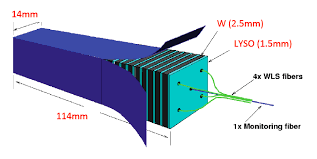
\includegraphics[width=0.6\linewidth]{figures/CMS/Upgrade/ShashlikTower.png}\\
\caption{A shashlik calorimeter tower. }
\label{fig:shashtower}
\end{figure}
is composed of 28 layers of Tungsten alternating with 29 layers of LYSO, where LYSO (LuYSiO$_5$(Ce)) is a high density (7.1 g/cm$^3$) scintillating material largely developed for use in particle detectors by Caltech \cite{Chen:2007bb}. The HGCAL is a sampling calorimeter that will be built from alternating lead and copper sampling layers, with signal readout from silicon photosensors. The HGCAL design is notable for its ability to provide longitudinal as well as lateral information about the distribution of energy deposited by high-energy particles.

In April-May of 2014 and July-August, 2014, test beam experiments were held at Fermilab at the M-Test facility~\cite{Fermi:T1041} to study and characterize a prototype module of the shashlik calorimeter (Figure \ref{fig:shashscatter} illustrates the prototype structure). 
\begin{figure}[h]\centering
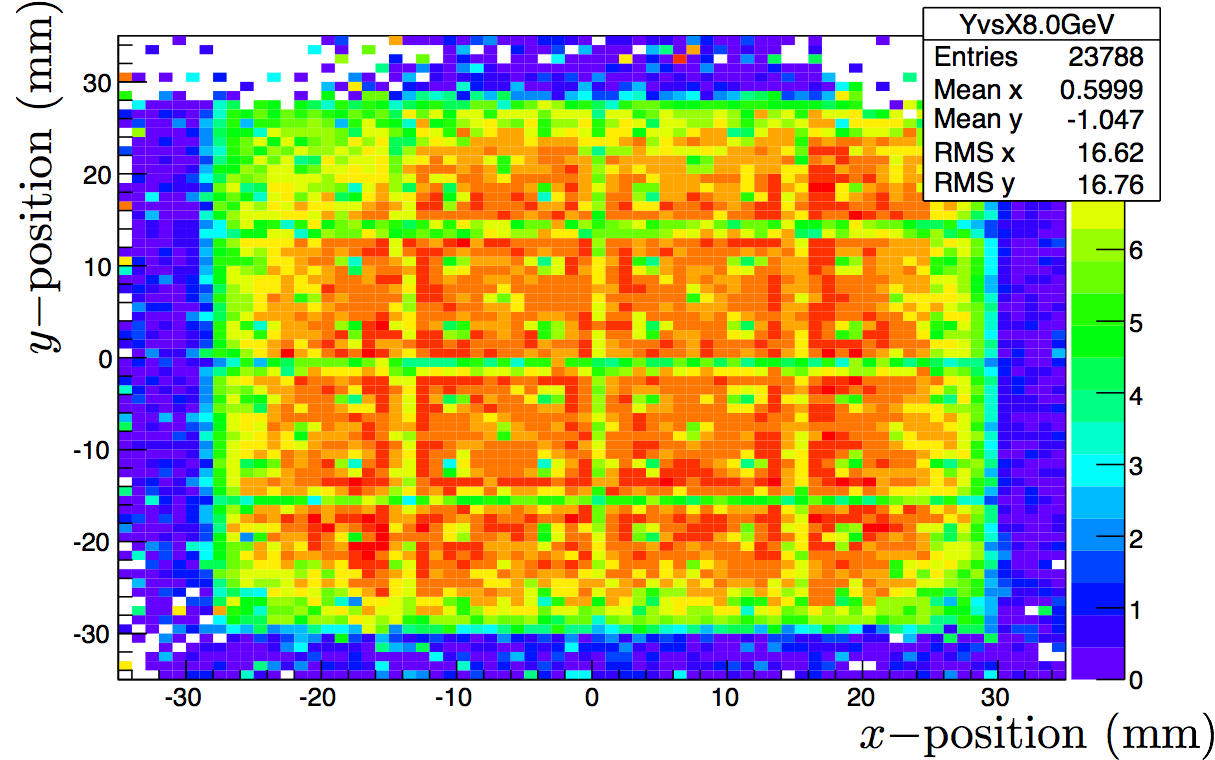
\includegraphics[width=0.6\linewidth]{figures/CMS/Upgrade/TopoMap.png}\\
\caption{A scatter plot of the accumulated track positions weighted by the in-time energy deposited in the shashlik tower, for a set of muon runs recorded in July, 2014. The $4\times4$ tower array structure, the gaps between towers, and the holes bored for the WLS fibers can be seen as green features.}
\label{fig:shashscatter}
\end{figure}
The testbeam facility provided access to beams of particles with an energy per particle ranging from 1 to 120 GeV. Several characteristics of the beam could be chosen in real time, such as the species of particles populating the beam, as well as the energy per particle.  The facility also provided the use of two wire chambers, which were used to determine the time and position of incident particles.The shashlik prototype consisted of a $4\times4$ array of towers, and each tower (Figure \ref{fig:shashtower})
\ref{fig:shashtower})
was read out by four wavelength-shifting (WLS) fibers fed longitudinally through the towers and connected to silicon photomultiplier sensors (SiPMs). 

While working help set up and manage the testbeams, I authored an interactive event display that was used to view data as it was being collected. The event display is a flexible, python-based program with a graphical user interface (GUI) that can be be used to view both live as well as stored data. The GUI is largely based on the TEve class of the Root software package \cite{Brun:1997pa}, which makes use of a slots and signals framework to enable communication between objects defined in the program. Signals carry information related to one or several user-defined objects, can be produced as a result of various actions taken by the user or from the data stream, while slots are a class of objects that are capable of receiving this information and initiating changes to their associated user-defined objects. For a concrete example, after processing the tracking information for a given event, the program produces a signal that is received by the module that projects a 3-dimensional event view, which is updated to display a set of tracks.

The event display contains several view panels, including 
\begin{itemize}
\item a heat map (color plot) of the maximum analog-to-digital count (ADC) recorded by each channel during an event in real space, as shown in Fig. \ref{fig:HeatMaps} (top);
\item a display of the readout and $\chi^2$ of the samples by channel, and a display of the pedestal noise, as shown in Fig. \ref{fig:HeatMaps}, (bottom);
\item a display of the pedestal noise by channel, where the pedestal is the expected number of ADC counts in the absence of any signal, as shown in Fig. \ref{fig:NoiseAndWires};
\item a view of the in time hits in the wire chambers, where ``in time'' refers to the criterion that the recorded time of the signal be consistent with the time of the recorded energy deposited in the calorimeter, as shown in Fig. \ref{fig:NoiseAndWires}, and
\item a 3-dimensional view of of the hits, tracks, wire chambers, and the shashlik calorimeter with color corresponding to the estimated energy deposited in each tower, as shown in Fig. \ref{fig:Shashlik3d}.
\end{itemize}
\begin{figure}[h]\centering
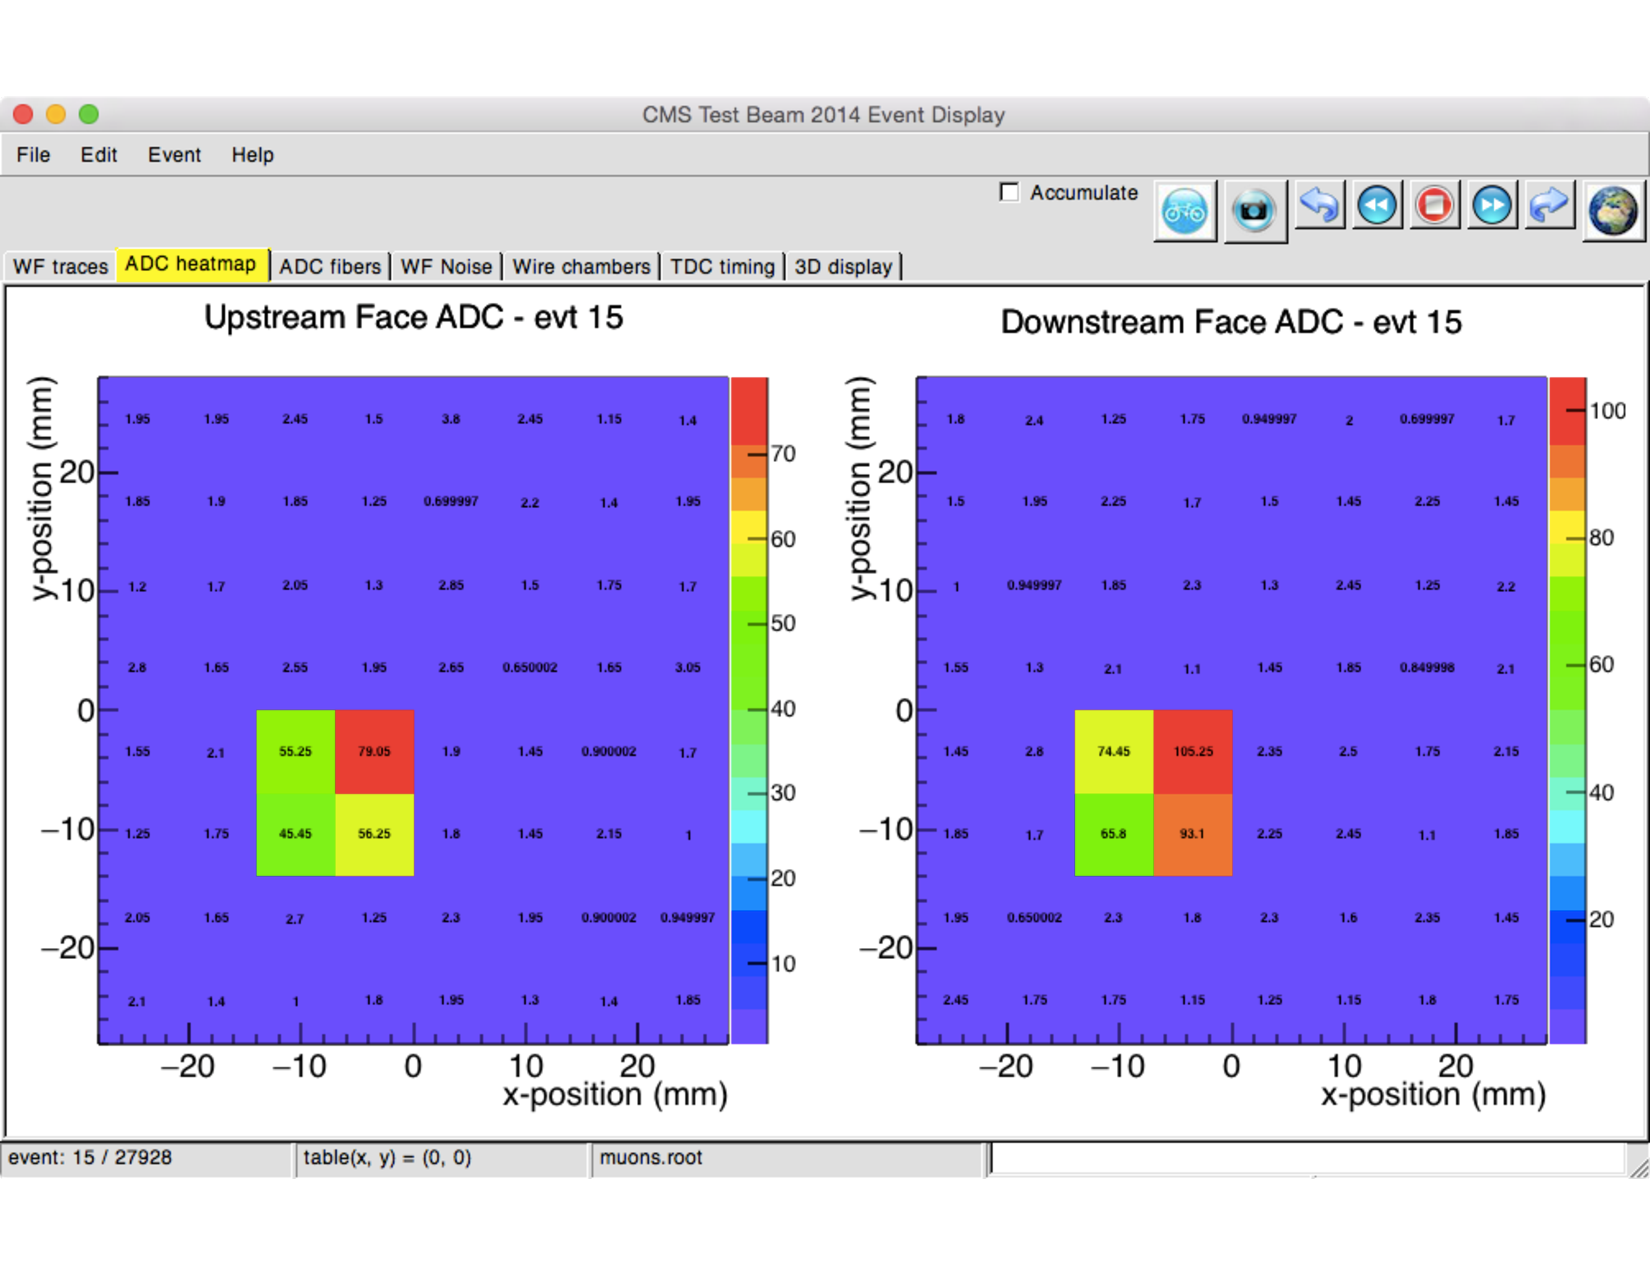
\includegraphics[width=0.85\linewidth]{figures/CMS/Upgrade/MuonHeatMap.pdf}\\
\vspace{-1cm}
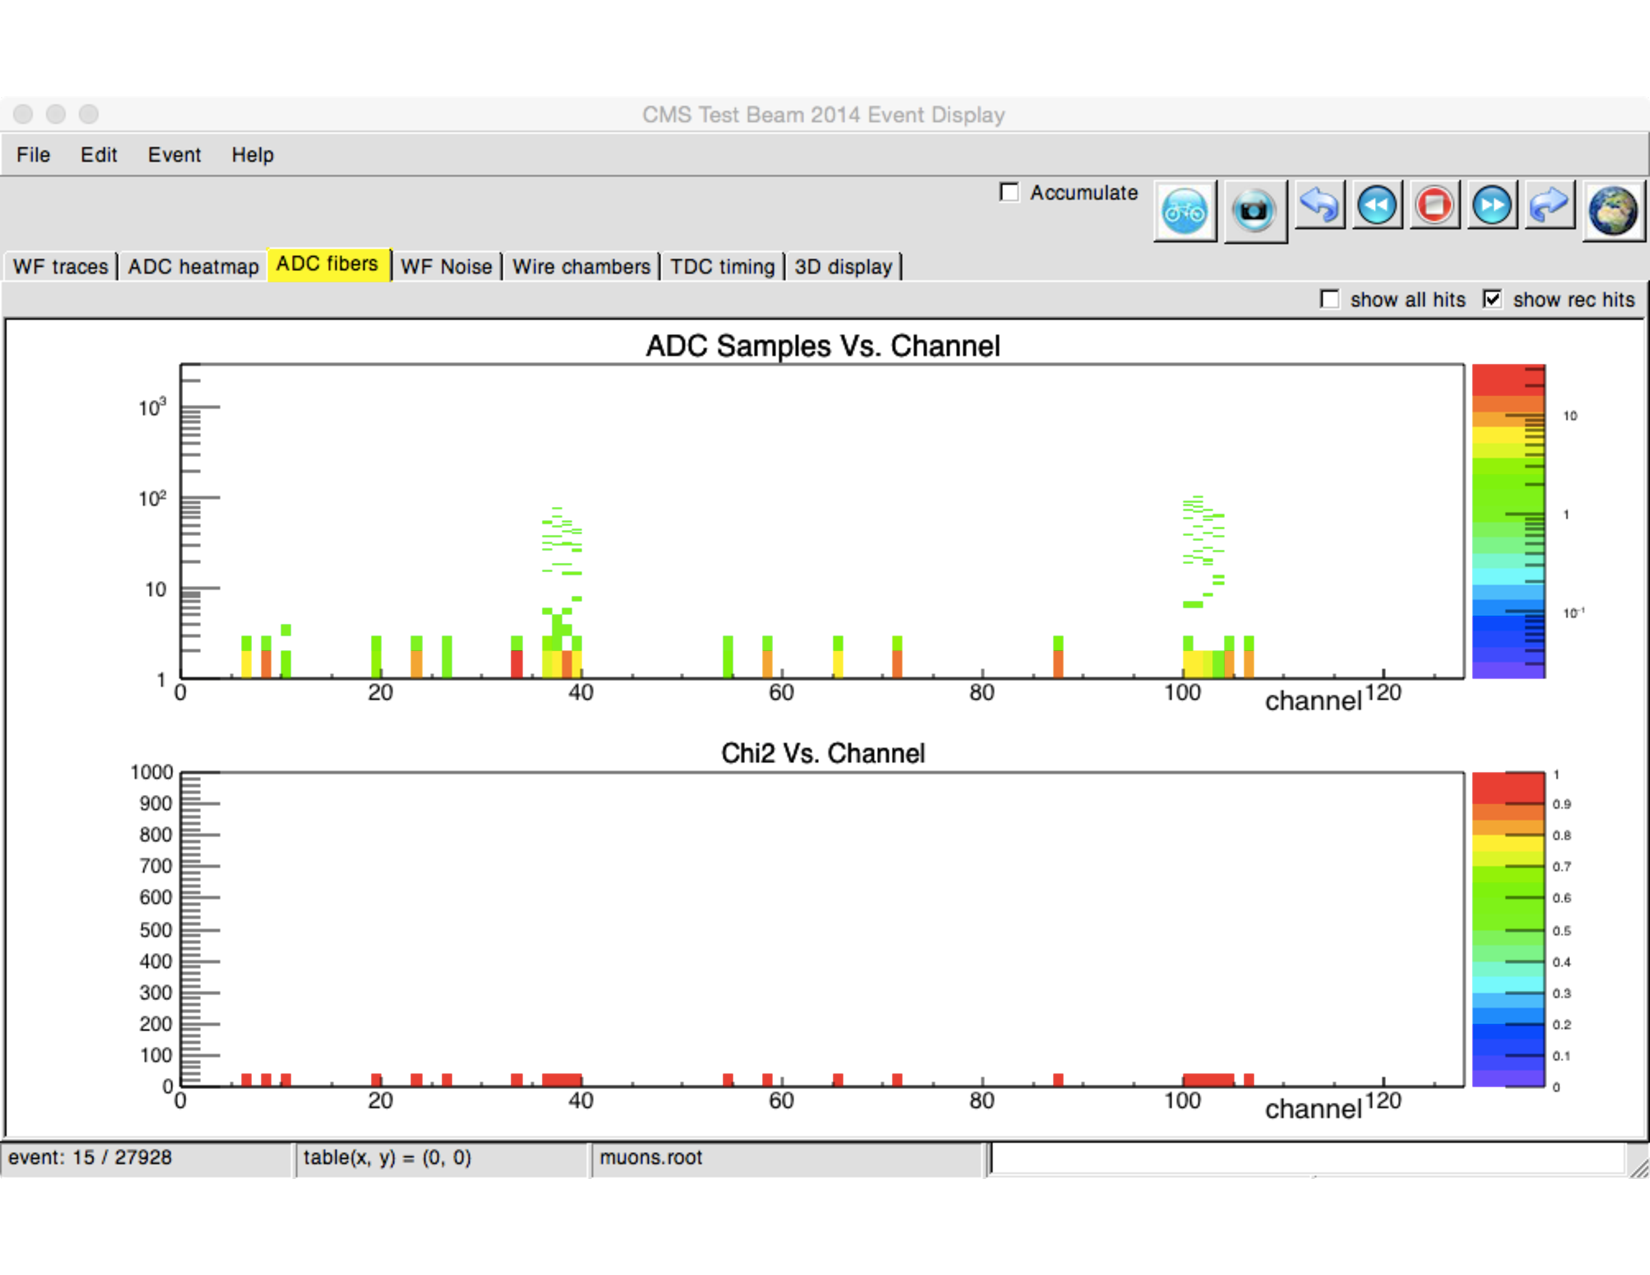
\includegraphics[width=0.85\linewidth]{figures/CMS/Upgrade/HealthyPulses.pdf}
\caption{Top: heat maps of the ADC counts recorded at the upstream and downstream faces of the shashlik module. Bottom: Diagnostic displays of channel-by-channel information from the shashlik module. The "Chi2 Vs. Channel" display is effective at revealing noisy channels, that is, channels with a large ADC count generated by electronic noise rather than a genuine particle signal.}
\label{fig:HeatMaps}
\end{figure}
\begin{figure}[h]\centering
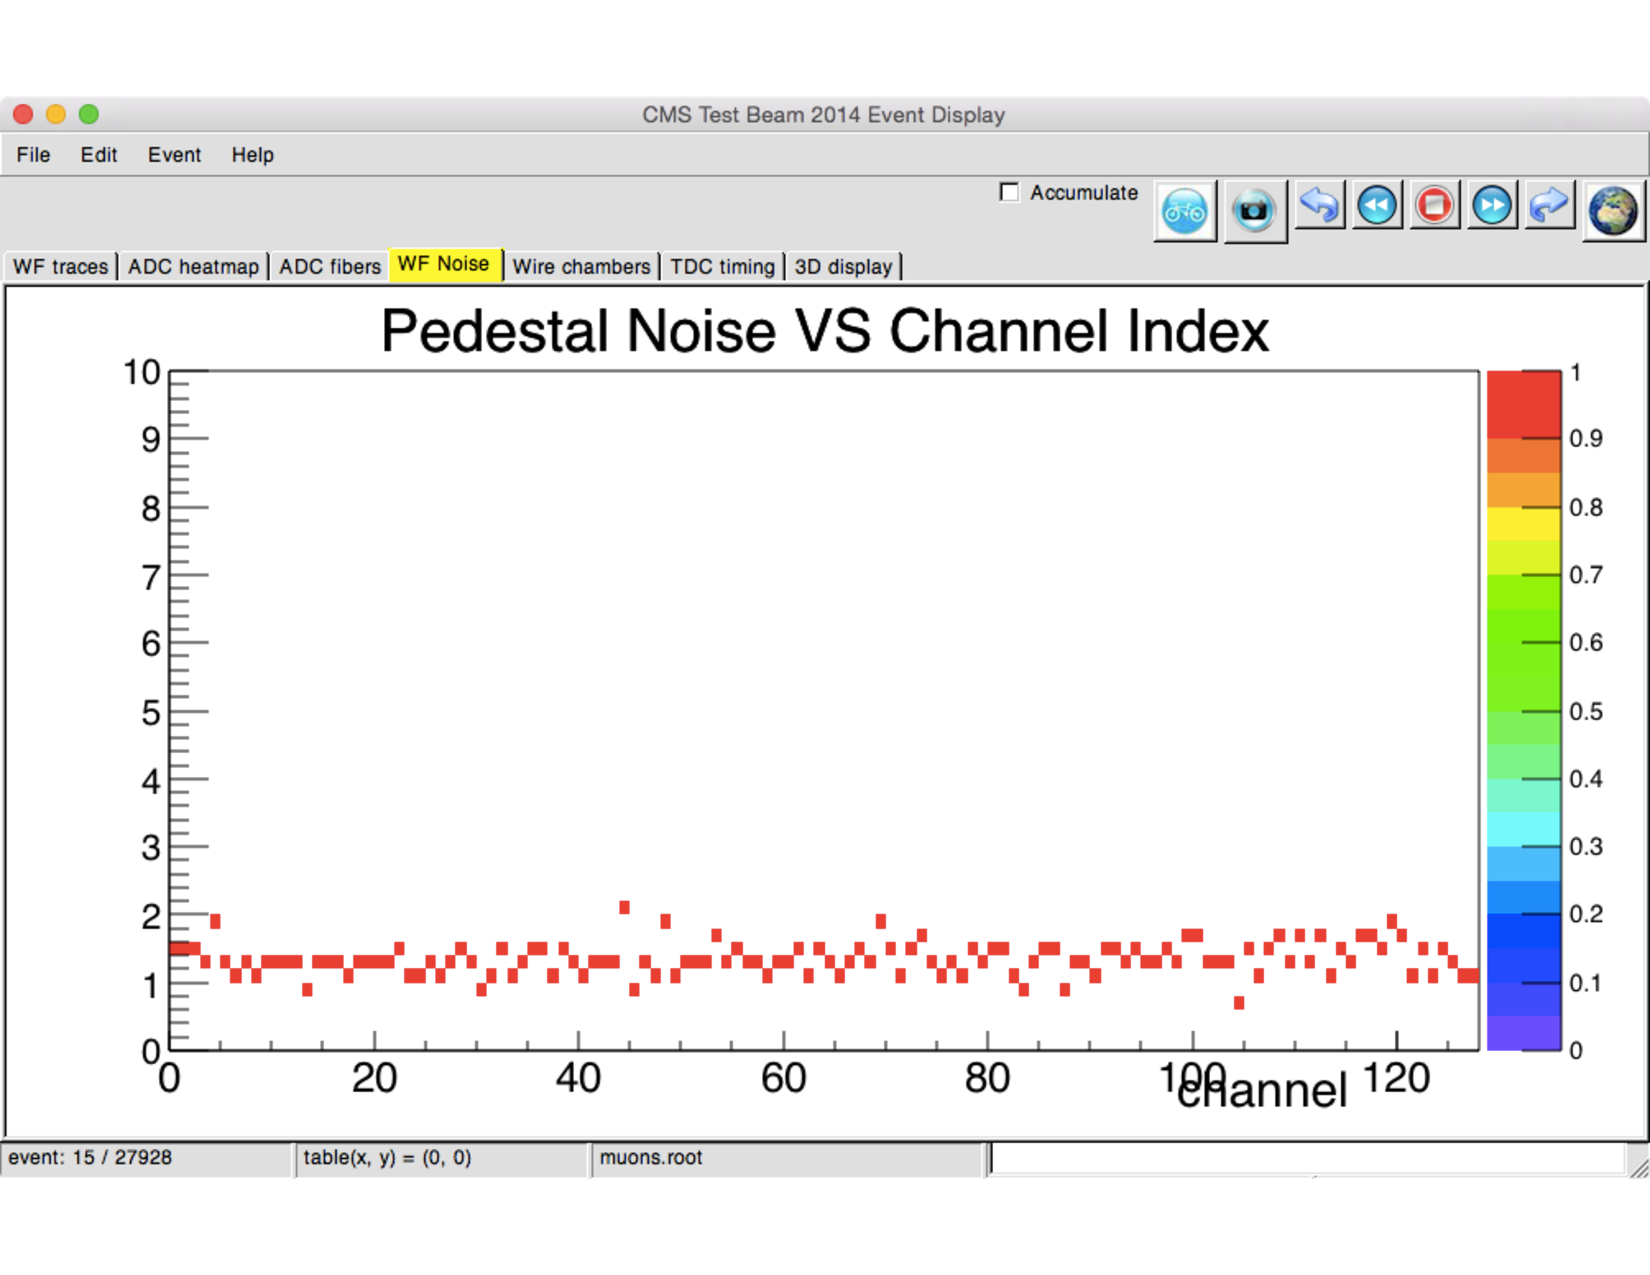
\includegraphics[width=0.8\linewidth]{figures/CMS/Upgrade/PedestalNoise.pdf}\\
\vspace{-1cm}
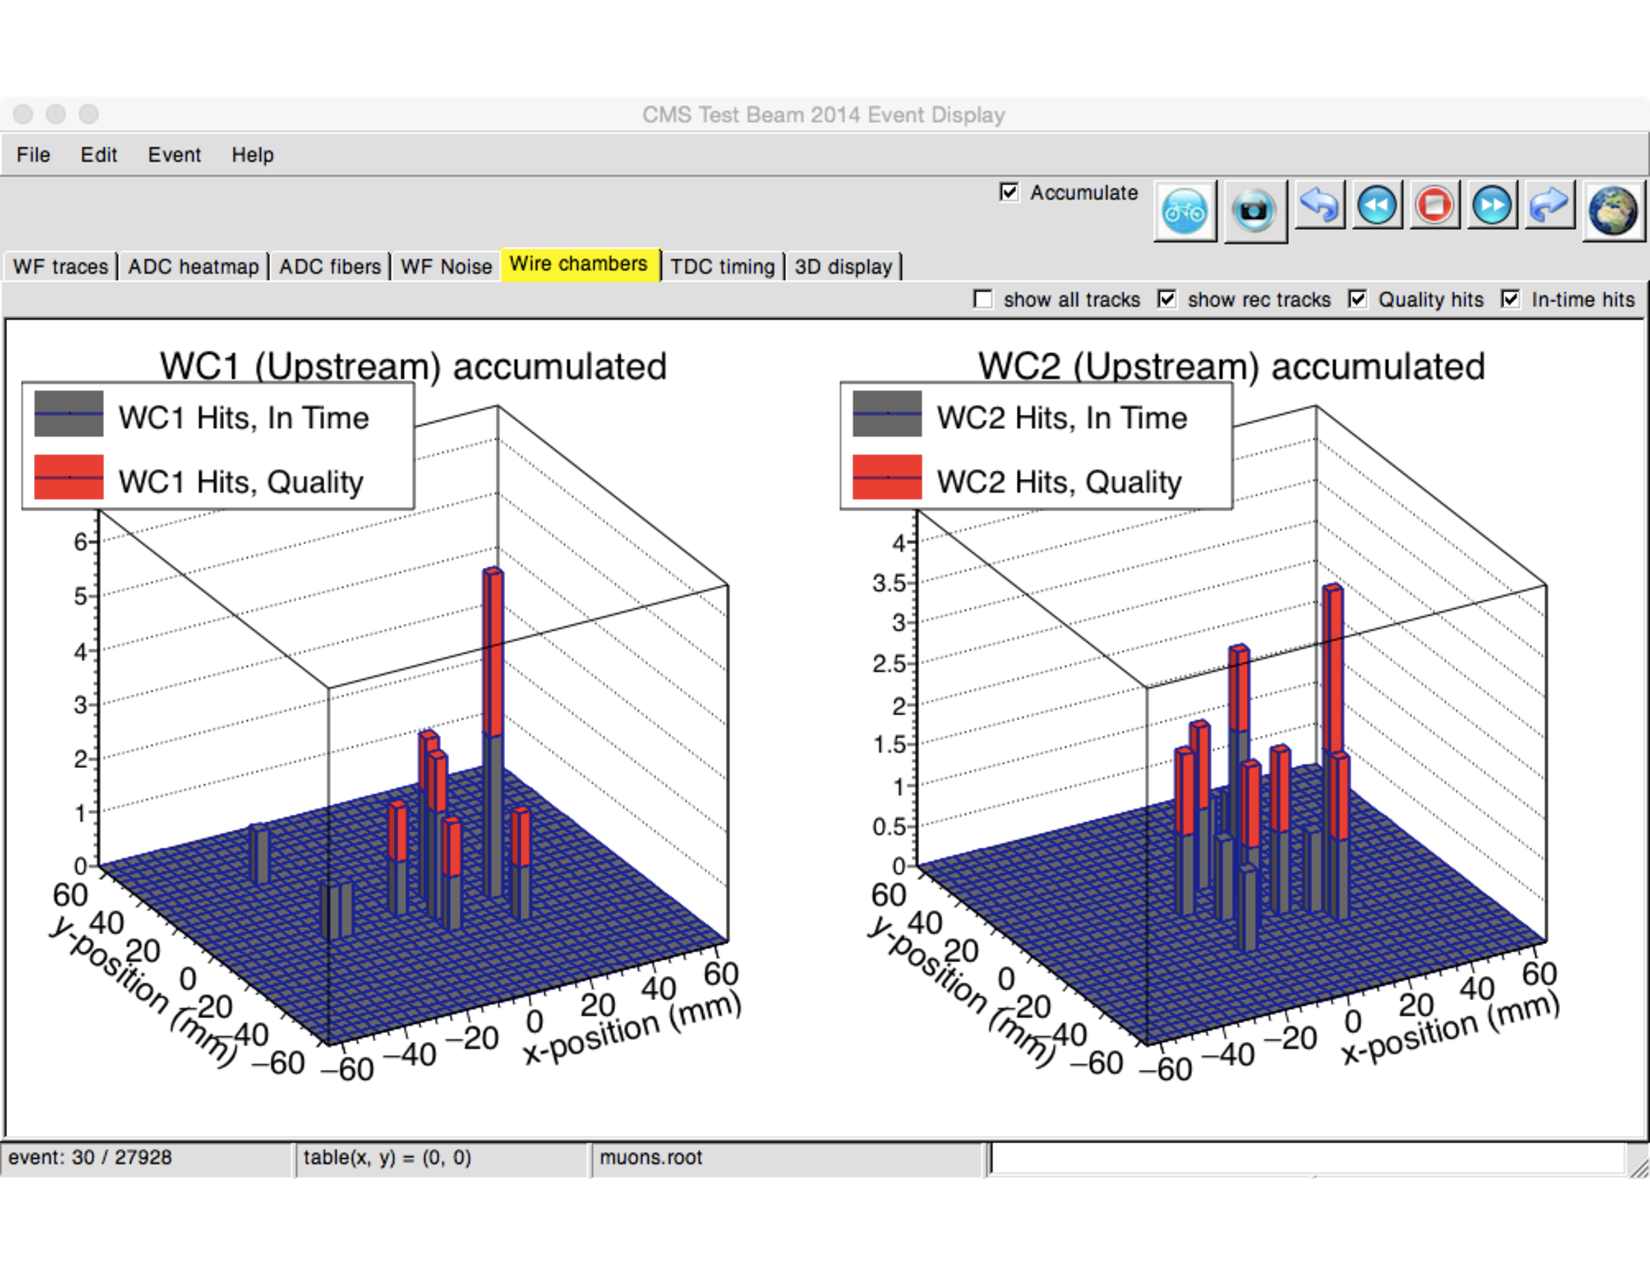
\includegraphics[width=0.8\linewidth]{figures/CMS/Upgrade/WireChambers.pdf}
\caption{Top: The pedestal noise by channel. Bottom: A scatter plot of the positions of accumulated hits and tracks recorded by the wire chambers; quality hits are colored red, and refer to hits consistent with a particle track.}
\label{fig:NoiseAndWires}
\end{figure}
\begin{figure}[h]\centering
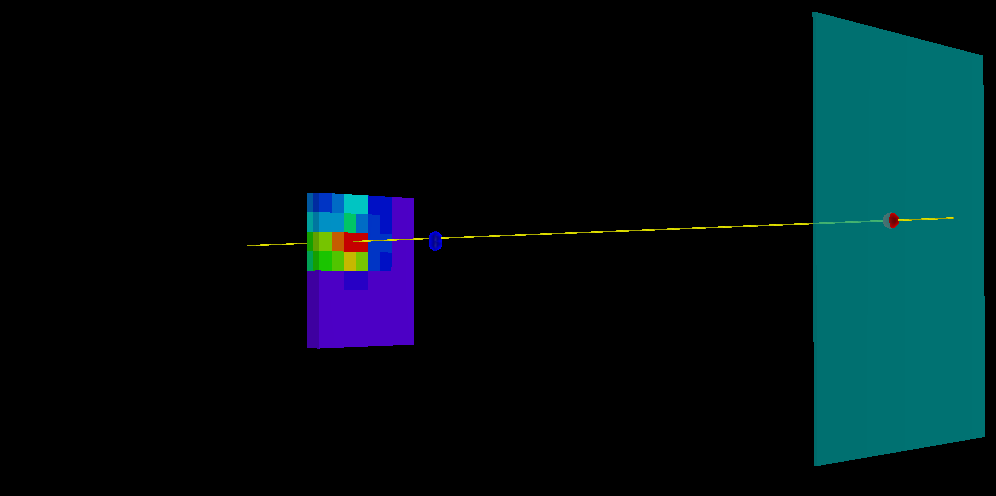
\includegraphics[width=0.8\linewidth]{figures/CMS/Upgrade/3D_50.png}\\
\vspace{0.8cm}
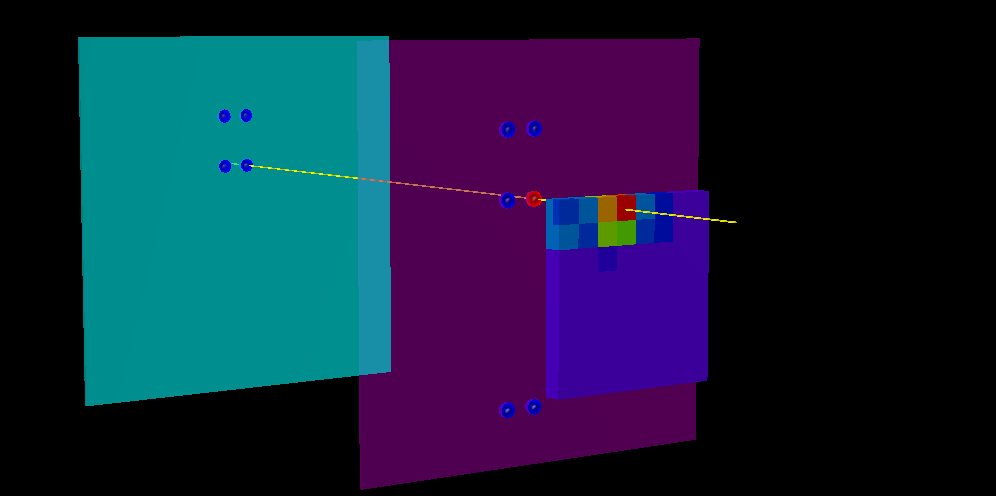
\includegraphics[width=0.8\linewidth]{figures/CMS/Upgrade/3D_14.png}
\vspace{0.8cm}
\caption{Three-dimensional views of reconstructed tracks and calorimetric energy deposits in events containing a 120 GeV proton. The view can be rotated by the user, allowing different viewing perspectives of the event, as illustrated in the top and bottom figures.}
\label{fig:Shashlik3d}
\end{figure}
\noindent
The event display has since been adopted for use at testbeam experiments dedicated to studying the HGCAL, where a prototype of the future calorimeter is being characterized. The software for the event display can be obtained at the url in Ref.~\cite{bib:EventDisplay}. 

\subsubsection{Jet/\MET analysis}
After testbeam operations, I and my colleague Arka Santra performed analysis of the data collected, as well as of simulated events. The energy resolution of jets in the CMS endcaps for various phases of the CMS detector are shown in Fig. \ref{fig:ShashlikResolution}.
\begin{figure}[h]
\centering
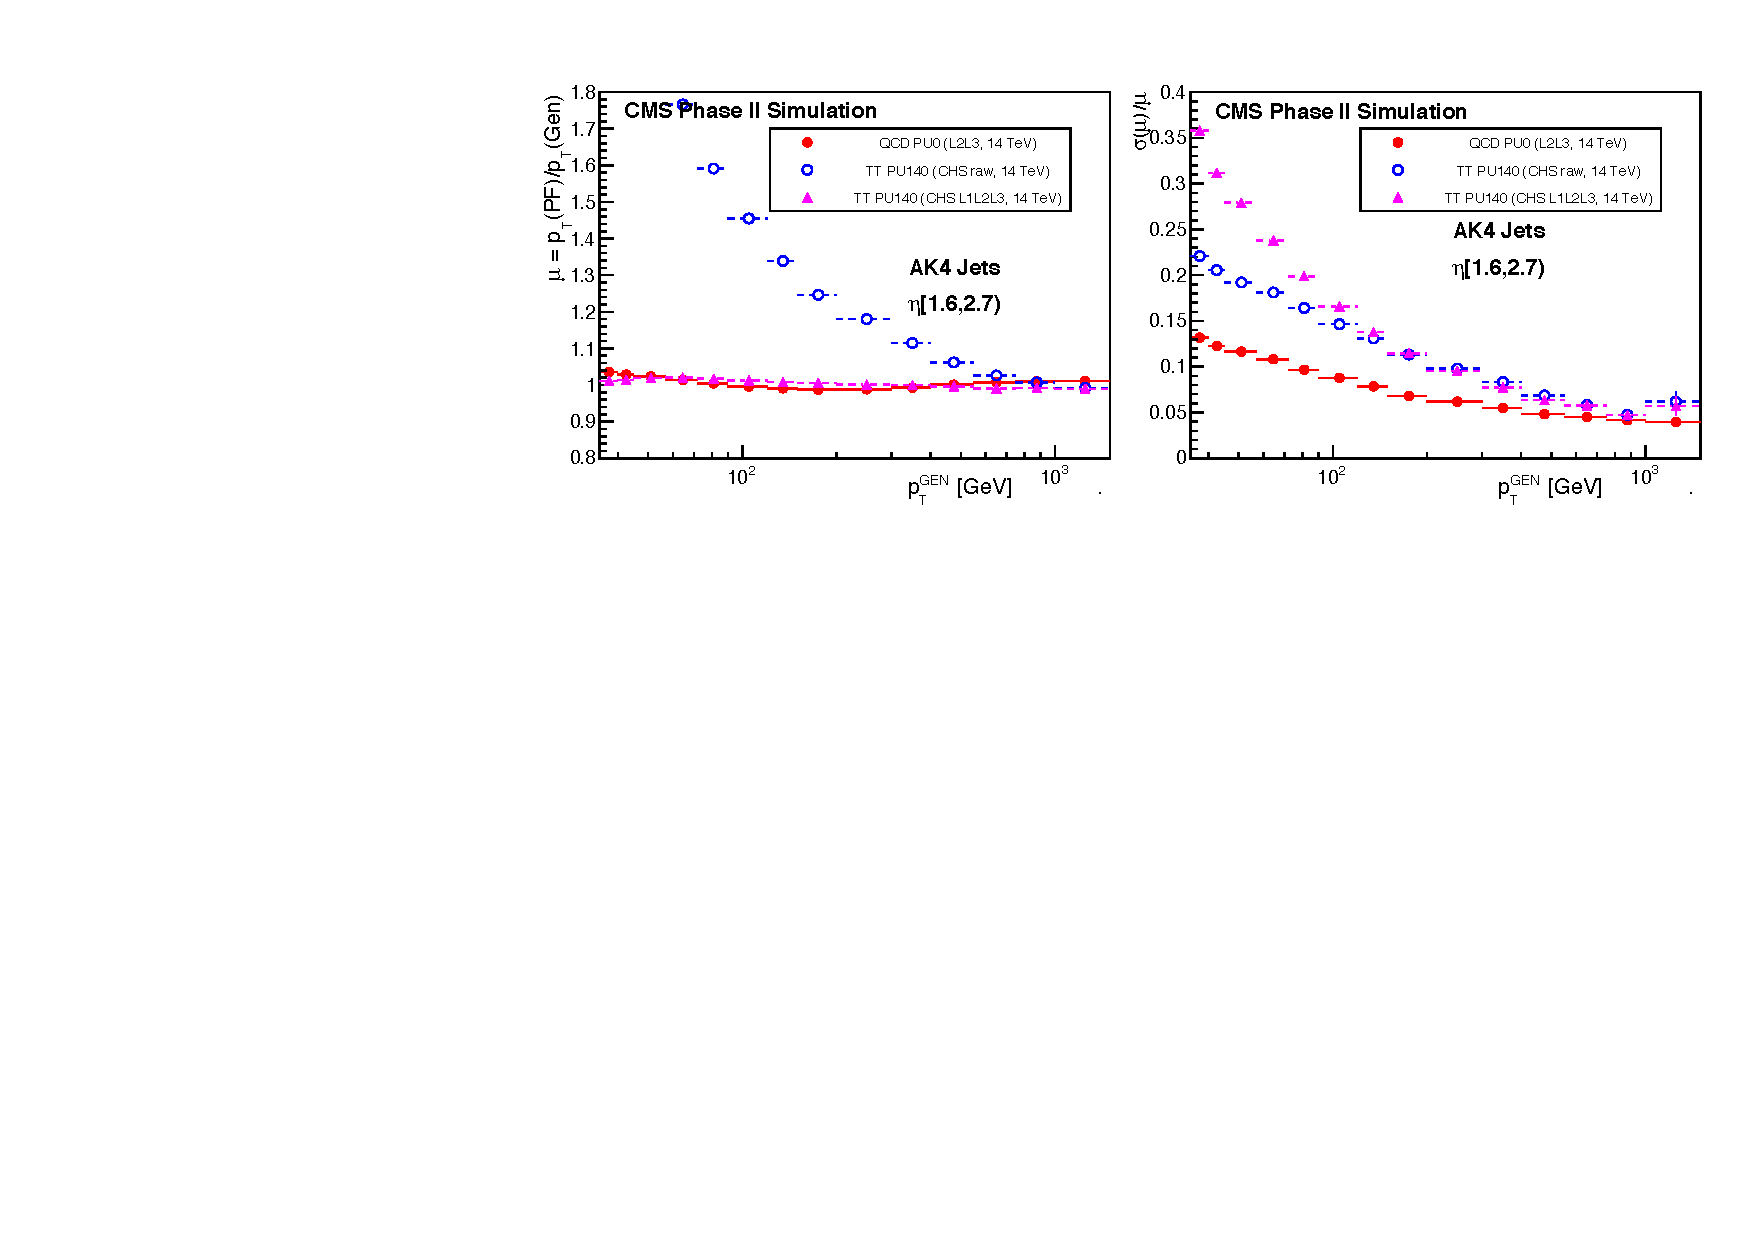
\includegraphics[width=0.9\linewidth]{figures/CMS/Upgrade/ChsJetPerformanceEndcapTT.pdf}
\caption{The jet response (left) and energy resolution (right) in the shashlik endcap as a function of simulated jet $p_T$ in a sample of simulated $t\bar{t}$ events. The red distributions correspond to the scenario without pile-up, and pink to that with pile-up of 140 (an average of 140 collisions per bunch crossing), which is the expected amount of pile-up during the post-Phase II LHC operations. }
\label{fig:ShashlikResolution}
\end{figure}
At large $p_T$, the energy resolution in PU 140 events is seen to drop below 10\%, indicating an excellent level of performance that surpasses that described in Ref.~\cite{Bilki:2015rla}.

\FloatBarrier





